\documentclass{article}

% Language setting
% Replace `english' with e.g. `spanish' to change the document language
\usepackage[english]{babel}

% Set page size and margins
% Replace `letterpaper' with`a4paper' for US/EU standard size
\usepackage[letterpaper,top=2cm,bottom=2cm,left=3cm,right=3cm,marginparwidth=1.75cm]{geometry}

% Useful packages
\usepackage{amsmath}
\usepackage{graphicx}
\usepackage[colorlinks=true, allcolors=blue]{hyperref}

\title{Data 102 Final Project Report}
\author{Jiaxin Li, Jiarui Luo, Jindi Chen, Jingqi Huang}
\date{\displaydate{December 13, 2021}}

\begin{document}
\maketitle


\setlength{\parindent}{0cm}
\section{Data Overview}

We use the data downloaded from Center for Disease Control and Prevention (\href{https://chronicdata.cdc.gov/Chronic-Disease-Inicators/U-S-Chronic-Disease-Indicators-CDI-/g4ie-h725}{CDC}). The data is a census over U.S. states across certain years on many topics. The first research question uses data from two filter dataset: \href{https://chronicdata.cdc.gov/Chronic-Disease-Indicators/U-S-Chronic-Disease-Indicators-Asthma/us8e-ubyj}{\textit{U.S. Chronic Disease Indicators: Asthma}}, and the other is \href{https://data.cdc.gov/Environmental-Health-Toxicology/Daily-Census-Tract-Level-PM2-5-Concentrations-2011/fcqm-xrf4}{\textit{Daily Census Tract-Level PM2.5 Concentrations}}. The second research question uses data from \href{https://chronicdata.cdc.gov/Chronic-Disease-Indicators/U-S-Chronic-Disease-Indicators-Cardiovascular-Dise/232j-jiq5}{\textit{U.S. Chronic Disease Indicators: Cardiovascular Disease}} and \href{https://chronicdata.cdc.gov/Chronic-Disease-Indicators/U-S-Chronic-Disease-Indicators-Tobacco/rrbt-bhen}{\textit{U.S. Chronic Disease Indicators: Tobacco}}. Non-adults who aged below 18 years old are excluded from part of the asthma dataset that relates to asthma prevalence, influenza vaccination rate, and pneumococcal vaccination rate as well as the tobacco dataset that includes smoking and smokeless tobacco consumption percentages. We also observe that while state is represented by state name in the asthma dataset, on the other hand, it is shown as state code in the PM2.5 dataset. Hence we introduce an external \href{https://www.census.gov/library/reference/code-lists/ansi/ansi-codes-for-states.html}{\textit{Statefips-to-Name dataset}} to help us merge the two datasets if needed in the following sections.

In terms of granularity, each row of the indicator dataset (asthma, cardiovascular and tobacco) shows the statistics of different questions for the population group stratified by state, year, and specific data value types. Each row of the PM2.5 dataset represents the mean predicted PM2.5 concentration and associated standard error at the city and daily level. The differences between the granularity of asthma and PM2.5 datasets imply that aggregation of the PM2.5 data will be needed if we want to connect the two datasets in the analysis and modeling sections. In the cardiovascular and tobacco datasets, however, granularity levels are similar, and therefore are easier to merge and compare. 

Since no information can be found about participants’ awareness on the CDC website, we assume that participants are unaware of the collection and use of their data. And as healthcare performances could affect the prevalence and mortality rate of chronic diseases, it will allow us to have a better picture of asthma and cardiovascular disease if healthcare quality in each state is included in the dataset.


\section{Research Question 1}
\textbf{After observing our datasets, we decide to do causal inference to estimate the effect of PM2.5 concentration on asthma prevalence and asthma mortality rate.}
While high PM2.5 level is generally considered as unhealthy, knowing its causal relationship to specific chronic disease like asthma allows us to have a better understanding of what “unhealthy” really means and raises public awareness of the severity of air quality issues. For instance, if high PM2.5 concentration is proven to cause asthma, then public authority like CDC will have more concrete as well as scientific evidence to issue regulations that control levels of particulate matter. 

\subsection{Exploratory Data Analysis}
\subsubsection{Data Cleaning}
For the following visualizations to be done, we aggregate the PM2.5 dataset to get average concentration, latitude, and longitude at state and yearly level. Then we merge the two datasets, using the external Statefips-to-Name dataset.

\subsubsection{Data Visualization and Analysis}
To find confounders and covariates of our causal inference, we first visualize the quantitative variable Year, categorical variable State, and their relationships to the PM2.5 and asthma. As the figure \ref{fig:figure20} shows, each subplot is one state with X axis being year, gold part being crude asthma prevalence rate, and blue part being the PM2.5 concentrations. Clearly, each state has its own asthma prevalence level and PM2.5 concentration level, which is possibly due to the differences in industrial development, medical performances, or environmental regulations among all the states. And we can also observe yearly differences in asthma prevalence and PM2.5 concentration. Since state and year affect both our treatment and outcome, they are considered as confounders of our causal inference. 

Then we graph two categorical variables, race and gender. As the figure \ref{fig:figure21} and figure \ref{fig:figure22} show, in every state, both asthma prevalence and asthma mortality rate are higher in the female group than the male group, indicating that gender is a covariate that we need to add to the model later. In terms of race, from figure \ref{fig:figure23} and figure \ref{fig:figure24}, it seems that asthma prevalence is highest in the multiracial and 
African American group and lowest in the Hispanic group, and we can still observe that asthma mortality rate is noticeably higher in black community than white community. Therefore, race is also a covariate that needs to be added to the modeling process. 

Finally, we visualize the quantitative variable latitude. The figure \ref{fig:figure25} and figure \ref{fig:figure26} show that as latitude increases, asthma tends to increase while the PM2.5 concentration tends to decrease. This finding validates latitude’s role as a confounder, as it affects both the treatment (PM2.5 concentration) and the outcome (asthma prevalence and asthma mortality rate). 

\subsection{Methods}
Since our data does not represent a randomized trial with randomly allocated treatment, we consider using the methods of matching, instrumental variables and two stage least squares, or inverse propensity weighting (IPW) to answer our first research question. Due to the limitations of not enough information to find appropriate instrumental variables and poor matching or curse of dimensionality caused by continuous confounders, we devise a propensity score model to control for observed confounders. If we assume that the only confounders of our problem are the ones in our dataset (year, state, latitude, and longitude),  the unconfoundedness assumption holds for the definition of the propensity score---it is the probability that a unit is treated conditioned on a particular set of confounders. No collider is detected in our dataset so the issue of colliders will not be addressed here. 
\subsubsection{Binarization}
We first binarize our treatment variable (PM2.5 concentration) so as to later estimate the average treatment effect (ATE). In other words, we transform the exact values of PM2.5 concentration rate into binary treatments xi (0 or 1), which indicates whether or not the PM2.5 concentration is relatively high. Referring to the current national limit for fine particulates set by the US Environmental Protection Agency (EPA), we initially use 12 µg/$m^3$ of air as the threshold. However, this threshold results in a serious unbalance between the treatment and control group: only 0.46\% of the data is in the treatment group. With the aim to balance both groups, we adopt the stricter threshold of 9 µg/$m^3$, which separates 54\% of the data into the treatment group (relatively high PM2.5 concentration: PM2.5 $>$ 9) and 46\% into the control group (relatively low PM2.5 concentration: 0 $\leq$ PM2.5 $\leq 9$). 
\subsubsection{IPW and ATE}
After binarization, we proceed to calculate the propensity scores and estimate the ATE. However, although both gender and race can possibly affect asthma prevalence and mortality rates as shown in the EDA section, due to the structure of the original CDC dataset, we cannot stratify the data on gender and race at once. As a result, we decide to stratify the data on gender or race separately. In addition, for asthma prevalence rates, we have both crude prevalence rates, age-adjusted prevalence rates recorded. It is not clear according to the information at hand which one is more appropriate for use as the outcome variable. Asthma mortality rates have a similar issue. We solve this problem by calculating 8 different ATEs using mortality and prevalence data, stratified by gender or race, with outcome variable represented as either crude rate or age-adjusted rate.

We estimate \^{e(x)} (the predicted probability that zi = 1) by fitting a logistic regression model that predicts zi from all the features xi at hand. Since we assume unconfoundedness, the IPW estimator of ATE is unbiased. We estimate treatment accounting for the propensity according to the function listed below:

\begin{figure}[h]\centering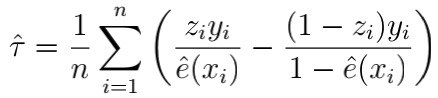
\includegraphics[width=0.25\textwidth]{formula.jpg}\end{figure}

\subsection{Conclusion}

\subsubsection{Model Result and Interpretation}
 \begin{figure}[h]\centering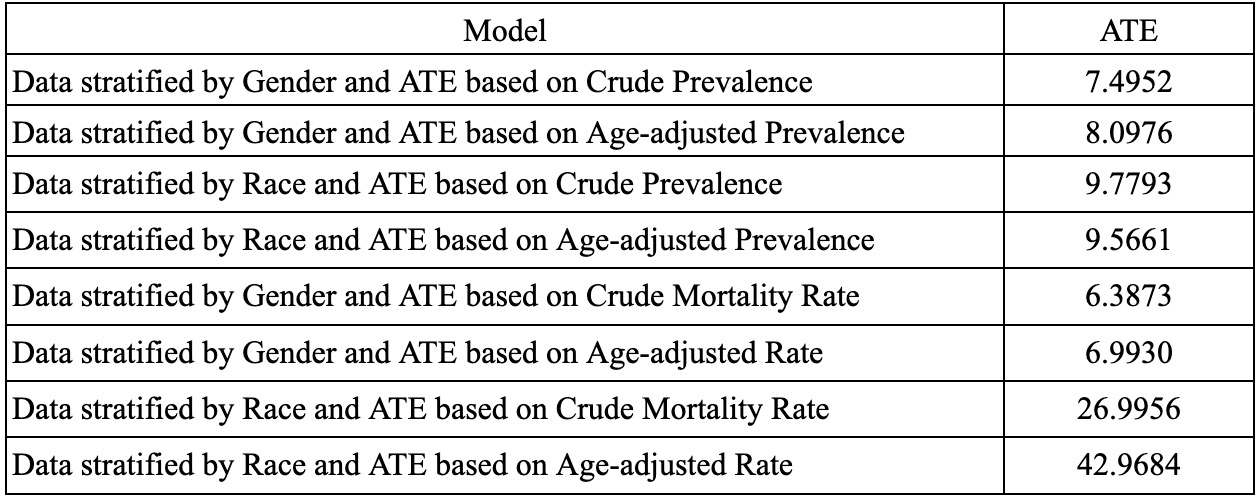
\includegraphics[width=0.85\textwidth]{Q1 Result Table.jpg} \end{figure}
 From the above table we can see that all of the eight estimates of the treatment effect are positive, which strongly indicates that the treatment, that is, higher PM2.5 concentration rates, has a causal effect on both asthma prevalence and asthma mortality rate. Specifically, \textbf{an increase of PM2.5 concentration will cause both Asthma prevalence rate and Asthma mortality rate to increase.}
 
 \subsubsection{Limitation and Discussion}
Although all eight ATEs suggest a positive causal relationship between PM2.5 concentration and asthma, this result only holds with the assumption that year, state, longitude, and latitude are the only confounders in our causal inference. However, the real world problem is much more complex than our model. Other confounders that are not included in the datasets, such as the development index, which both affects PM2.5 concentration (better air quality in more developed areas due to more strict regulations) and asthma (high healthcare quality that controls asthma better in more developed areas), also affect the performance of our causal inference process. On the other hand, according to the CDC, there are other covariates that also trigger asthma like respiratory syncytial virus (RSV) and dust mites, and having more confounders in our model may help us validate and quantify the causal effect. Moreover, although our data and results provide intuitions on the statewide causal relationship between PM2.5 and asthma, it is also worth noting that PM2.5 concentration and other variables can be unevenly distributed within each state. Thus, having access to these variables in smaller geographical scales may generate more accurate results. Finally, even though we have successfully shown the positive causal relationship between PM2.5 concentration and asthma prevalence and mortality and is accordant to intuitive sense, further research may be needed to provide detailed reasoning about the mechanism of PM2.5 affecting asthma. 



\section{Research Question 2}
\textbf{In this section, we aim to create models using Generalized Linear Models (GLMs) and Non-parametric Models to predict the risk level of cardiovascular disease mortality based on the use of tobacco.} We believe that this research question could shed some light on how tobacco consumption and regulation impact people's cardiovascular health, and therefore if applied on real-world data, the models could advise residents and government to make decisions regarding tobacco use and regulation. Since we are uncertain about whether the true relationship between the two variables are linear, we choose to use both GLM and non-parametric methods to fit out data. 


\subsection{Exploratory Data Analysis}
\subsubsection{Data Cleaning}
The cardiovascular dataset contains records of survey questions from 2010 to 2019 across states and the tobacco dataset contains survey records from 2007 to 2019 in a similar format. From a basic overview, two crucial problems to deal with are NaN values and the selection of appropriate survey results for the research question. 

Firstly, there exist 28.52\% NaN data values for cardiovascular dataset, and 35.04\% for tobacco dataset. We delete rows with NaN values since at this stage we lack a well-rounded understanding of the data collection method and dataset content such that we cannot generate reasonable estimates to fill in NaN values at hindsight. 
There are 18 questions in cardiovascular dataset (Table~\ref{tab:questionIdTable}) and 16 in tobacco dataset (Table~\ref{tab:questionIdTable2}). We notice that the original dataset is stratified over three categories of gender, race, and overall. Since the primary goal of this research is to understand the general association of tobacco and cardiovascular mortality, we focus on the overall stratification category. 

From data cleaning, we recognize that our decisions to drop NaN values and focus on overall stratification category could result in a smaller amount of data for modeling and also a more general model that could fail to represent specific gender and race. We should be aware of the limitations when applying them to the reality.  

\subsubsection{Data Visualization and Analysis}

In this section, we aim to understand the content of the dataset to guide the model tuning process. 

In Figure \ref{fig:figure1}, we try to learn the general trend of cardiovascular mortality (cases per 100,000) across state and year. In general, the darker points that represent recent years are at the lower end for mortality, but the mortality levels vary significantly across states. For tobacco dataset, Figure \ref{fig:figure3} is generated to check the trend of current smoking among adults. In general, the darker points are at lower end, meaning that tobacco usage is lower for recent years across states.

Further on, in Figure \ref{fig:figure2}, we attempt to understand how tobacco retail license requirement impacts cardiovascular mortality, which helps with understanding the relationship of tobacco and cardiovascular mortality from the seller's side. However, almost no correlation can be observed simply conditioning on license requirement. For instance, Minnesota and Mississippi both require license but have sharply different mortality rate. Therefore, the next direction to investigate is on the consumer's side, using current smoking percentage. In Figure \ref{fig:figureset}, across all subplots for different years each state, it seems that both lines of current smoking adult percentage and cardiovascular mortality are decreasing concurrently as time evolves. Still, two states with similar smoker percentage can have very different mortality rate, such as New Jersey and New Hampshire, meaning that other confounders could be in effect. Lastly, the impact of smoker percentage on mortality can vary drastically across states. Therefore, we will treat each state's yearly data as different individuals for model input to account for this observation. 

\subsection{Feature Engineering}
From histogram of cardiovascular mortality in \ref{fig:figure5}, we notice the shape of double-peak curve centering on 200 and 250 (cases per 100,000) with a right skewed tail. We are curious if the two peaks actually corresponds with  states being tobacco popular and non-popular. From histogram of current smoking adult percentage, current smokeless tobacco use and sales of cigarette packs (Figure \ref{fig:figure6}, \ref{fig:figure7}, \ref{fig:figure8}, \ref{fig:figure9}), we roughly observe slightly right skewed normal curves. It is possible that these quantitative variables contribute to mortality and resulted in the double normal peak histogram. 

Juxtaposing current smoking adult percentage and cardiovascular mortality in original and standard unit in Figure \ref{fig:figure10} and \ref{fig:figure11}, we observe the positive association between smoking percentage and mortality across smoking and smokeless tobacco. With these  understandings, we proceed with features related to tobacco policy and usage for model input (see Table~\ref{tab:featurechosen}). The intuition is that higher tobacco usage leads to higher mortality, and regulation decreases mortality by setting limits on tobacco consumption. 

\subsection{Methods}
We try to fit models to predict overall cardiovascular mortality with tobacco usage. Features chosen and reasons are shown in above section.

For GLM, we use both Frequentist GLM and Bayesiam GLM. The assumption made for GLMs is that the underlying true association between tobacco and mortality is linear. We use four Frequentist GLM models, which are Poisson, Gaussian, Gamma, and Invert Gaussian. Difference in mean (220.29) and variance (1091.01) of the dataset indicates that Poisson may not be a suitable option. Since the histogram of cardiovascular mortality skewed to the right, we deliberately pick Bayesian GLMs that could capture such tendency, which are Gaussian, Gaussian with logarithmic output, Poisson, and Negative Binomial. 

For nonparametric models, we use K-Nearest-Neighbor(KNN), Random Forest and Neural Network to fit the model and record the performance. To avoid over-fitting the training data and acquiring more robust performance in testing data, we use random forest instead of decision tree. In non-parametric models, we make no assumption about the distribution of the data and the coefficients. 

We split the prepared data into train dataset and test dataset, and evaluate models performance mainly by comparing test errors. 

\subsection{Results}
\subsubsection{GLM}
\paragraph{Frequentist GLM:}
From Table~\ref{tab:freqglmsummary}, three goodness of fit indices indicate that all methods are poor fits of the data. Log-likelihoods are extremely negative, and deviance and Chi2 are very close to 0, which means that it is very unlikely under each model for the data to appear. The training and test errors are quite similar, with Frequentist Gamma GLM having the least in both. In addition from Table~\ref{tab:freqglmcoeff}, the model coefficient estimates are mostly close to zero.  Therefore, we proceed to Bayesian GLMs for better fit. 
\paragraph{Bayesian GLM:}
For Bayesian Gaussian GLM in Figure \ref{fig:figure12}, this model adjusts for the double-peak pattern by vertically peaking in between the two peaks. With logarithmic output, Figure \ref{fig:figure14} indicates that the model predicts closer to the taller peak of the mortality histogram vertically. For Bayesian Poisson GLM, Figure \ref{fig:figure16} indicates that this model generating a distribution that horizontally accounts for both peaks by the boundaries. The Bayesian Negative Binomial GLM contains both peaks by the boundaries horizontally and adjusts for the vertical distance between two peaks in Figure \ref{fig:figure18}.

Across all models in Figure \ref{fig:figure13}, \ref{fig:figure15}, \ref{fig:figure17}, and \ref{fig:figure19}, only current smoking adult percentage and retail license requirement have credible intervals that do not contain zero, showing high level of uncertainty. The estimated coefficient for current smoking adult percentage coefficient is 6.09, 0.0269, 0.0277, and 0.0271 for Gaussian, Gaussian with logarithmic output, Poisson, and Negative Binomial. The estimated coefficient for retail license policy in the same model sequence is 11.4, 0.0469, 0.0485, and 0.0499. 

It is notable that except for Gaussian, all coefficient intervals are much tighter, raising risk for over confidence. It can be observed that Poisson GLM pays less attention to outliers and therefore is over confident but Negative Binomial GLM does not substantially improve this issue. 

\paragraph{GLM Model Summary:}
From Table~\ref{tab:glmerrorsummary}, the best model across all GLMs is Bayesian Gaussian GLM with Logarithmic Output by least test error of 26.24.  
For model method, we notice that all GLMs must make trade-offs due to linear assumption to account for the double-peak shape of the output and therefore have unanimously greater error. We then proceed to investigate non-parametric models that extend this linear limitation. 

\subsubsection{Non-parametric Model}
From Table~\ref{tab:nonparamerrorsummary}, it can be observed that the training error increases with Random Forest, Neural Network, and KNN(k=3), while the test error increases with Neural Network, Random Forest and KNN(k=3). Therefore, with empirical results, the best model is Neural Network, with the lowest test error of 19.28 while having relatively low training error of 16.31. 

\subsubsection{Model Result Summary}
As we have explained why specific models stood out among GLMs and non-parametric models, we now attempt to compare all models' performance in Table~\ref{tab:allmodeltesterro}. Empirically, Neural Network outperforms other models by test error of 19.38, which is consistent with our prediction stated above. 

\subsection{Discussion}
\subsubsection{Model Result Interpretation}

In GLM section, we consistently observe bad model fits or insignificant coefficients. Although the right-skewed histograms of input features show great potential for continuous linear models to fit the output distribution, it is actually inappropriate to use continuous models to characterize the reality data. The reason is that, for all features, it is quite impossible to have a long right tail that theoretical distributions possess, which makes continuous modeling of the right tail very imprecise. Longer right tails would mean in reality to have extreme values. For instance, it is quite implausible to have 9,000 cases of mortality among 10,000 people. Therefore, the actual mean is always much lower due to this restriction. This fact causes all models to generate visualizations that are very close to what we could picture in mind for the observed data, but have numerically bad fit due to the limitation of infeasible outliers to get larger mean. For interpretation, we notice surprisingly from coefficient estimations that the effect of smoking percentage and regulation are both positive on mortality, with regulation having a even larger positive impact. The model results seem to be partially different from former belief that, increase in current smoker percentage should lead to increase in mortality, but increase in regulation should associate with decrease in mortality. 

For non-parametric models, KNN works badly for training and test error because we have many categorical features that consist of ones and zeros, which makes it much harder to group neighbors by only two possible values. In addition, decision trees can be impacted negatively if there exists noisy data points, making the training model to have strange corners and twists to perfectly fit the noise. This could be the potential reason why Random Forest fails to perform ideally. Neural networks use non-linear activation functions to deal with the complex nature of the interaction among input and output features. Empirically we have found this model to have the best test error with relatively good training error, and due to the difficulty interpreting non-parametric models, we cannot perform contextual analysis of the result from the Neural Network model. 

\subsubsection{Limitation and Discussion}
Despite we do pick the best model from  experiments, we are still very unsure about feasibility to expand the model application to reality future datasets. For instance, with Bayesian GLMs, we notice that 4 out of 6 features input have coefficient credible intervals that contain zero, and such level of uncertainty calls the future model applications into question. For neural networks similarly, the test error has been optimized with max iteration of 50,000, resulting in a possibly overtrained network that could fail to generalize well with new data. 

We recognize the limitations of the models and the most important one of them is the training data availability. We notice in the dataset that, some survey questions were conducted in non consecutive years, and survey questions differ in the time they were handed out. So when we outer join datasets for model tuning, there are a lot of NaN values that are later dropped. If we have better data collection methods and can acquire data for survey questions during concurrent and consecutive time intervals, we could have a more robust training dataset. Also, there exists much room for improvement in light of the many foreseeable confounders. As we point out in EDA, we recognize that time and state can be important confounders. With current available data, we actually used One-Hot-Encoder to account for time and state. But the resulting model will be heavily dominated by the effect of time and state, such that the effect of tobacco on cardiovascular mortality is almost minimal, with close to zero and statistical insignificant coefficient estimates. Therefore, we might further need to consider instrumental variables or Two-Stage-Least-Squares to peel off the effect of time and state to investigate and focus on effect of tobacco. In addition, it would be more helpful if we are able to obtain data such as the geographic average socio-economic situation, healthcare related information, etc. to investigate more possible confounders. 

\subsection{Conclusion}
To summarize the key findings, we found that in accordance to common belief, an increase in one unit of tobacco smoking adult percentage will lead to a 0.0269 increase of logarithmic cardiovascular mortality (cases per 100,000). Contrary to common belief, having tobacco retail license requirement will lead to an average 0.0469 increase of logarithmic cardiovascular mortality (cases per 100,000). The hypothetical interpretation is that, with more sophisticated regulations, the tobacco market is more well-regulated and open to lucrative business, and therefore boosts tobacco consumption that leads to greater cardiovascular mortality. This hypothesis requires further causal inference efforts to validate. 

\subsubsection{Future Recommendation}
Firstly, as stated in Limitation and Discussion section, more robust data is needed to improve the model performance by accounting for confounders such as demographic information such as gender, race, state, and time, and social conditions such as socio-economic status, healthcare. In this way, a better model that is more confident to be applicable to real-world future data can be tuned to achieve generality to specific groups of people.

Based on the key findings of this paper, we believe that the surprising positive association of tobacco regulation and cardiovascular mortality should be presented to the government to guide their policy-making process. If we could characterize the causal relationships via better modeling, we could advise the ideal level of tobacco regulations to decrease cardiovascular mortality.

\newpage
\appendix

\section{References}
Krstić, Goran. “Asthma Prevalence Associated with Geographical Latitude and Regional Insolation in the United States of America and Australia.” PLoS ONE, vol. 6, no. 4, Apr. 2011, p. e18492. PubMed Central, \href{https://www.ncbi.nlm.nih.gov/pmc/articles/PMC3072993/}{https://doi.org/10.1371/journal.pone.0018492}.


US EPA, OAR. National Ambient Air Quality Standards (NAAQS) for PM. 13 Apr. 2020, \href{https://www.ncbi.nlm.nih.gov/pmc/articles/PMC3072993/}{https://www.epa.gov/pm-pollution/national-ambient-air-quality-standards-naaqs-pm}.

CDC. “Learn What Could Be Triggering Your Asthma Attacks.” Centers for Disease Control and Prevention, 21 Aug. 2020, \href{https://www.cdc.gov/asthma/triggers.html}{https://www.cdc.gov/asthma/triggers.html}.


% \newpage
\section{Tables and Graphs}

\begin{table}[h]
\caption{\label{tab:questionIdTable}Cardiovascular Possible Question Excerpt}
\centering
\begin{tabular}{m|m}
ID & Question \\\hline
CVD1\_1 & Mortality from total cardiovascular diseases \\
CVD1\_2 & Mortality from diseases of the heart \\
CVD1\_3 & Mortality from coronary heart disease \\ 
... & ...
\end{tabular}
\end{table}

\begin{table}[h]
\caption{\label{tab:questionIdTable2}Tobacco Possible Question Excerpt}
\centering
\begin{tabular}{m|m}
ID & Question \\\hline
TOB1\_1 & Current cigarette smoking among youth \\
TOB1\_2 & Current smoking among adults aged $\geq$ 18 years \\
TOB2\_2 & Current smokeless tobacco use among adults aged $\geq$ 18 years \\
TOB5\_0 & States with strong polices that require retail licenses to sell tobacco products \\
... & ...
\end{tabular}
\end{table}

\begin{table}[h]
\caption{\label{tab:featurechosen}Features for the Model}
\centering
\begin{tabular}{m|m|m}
ID & Content & Type \\\hline
TOB1\_2 & Percentage of current smoking adults & Quantitative\\
TOB2\_2 & Percentage of current smokeless tobacco adults & Quantitative\\
TOB4\_0, TOB5\_0, TOB7\_0 & Whether has regulations & Categorical\\ 
TOB10\_0 & Sales of tobacco (pack sales per capita) & Quantitative
\end{tabular}
\end{table}

\begin{table}[h]
\caption{\label{tab:freqglmsummary}Summary for Frequentist GLM}
\centering
\begin{tabular}{m|m|m|m|m|m}
Method & Likelihood & Deviance & Chi2 & Training Error & Test Error \\\hline
Frequentist Gaussian GLM & -649.84 & 78484 & 7.85e+04 & 23.51 & 26.57\\
Frequentist Gamma GLM & -642.97 & 1.4835 & 1.50 & 23.15 & 26.45\\
Frequentist Inverse Gaussian GLM & -641.42 & 0.0066 & 0.00672 & 23.28 & 26.80\\ 
\end{tabular}
\end{table}

\begin{table}[h]
\caption{\label{tab:freqglmcoeff}Coefficients for Frequentist GLM}
\centering
\begin{tabular}{m|m|m|m|m|m|m}
Method & TOB1\_2 & TOB2\_2 & TOB4\_0 & TOB5\_0 & TOB7\_0 & TOB10\_0 \\\hline
Frequentist Gaussian GLM & 6.0866 & 0.3934 & 4.8318 & 11.4912 & -12.7946 & 0.0440 \\
Frequentist Gamma GLM & -0.0001 & 4.573e-08 & -8.011e-05 & -0.0002 & 0.0004 & -8.481e-07 \\
Frequentist Inverse Gaussian GLM & -1.096e-06  & 3.508e-08 & 7.85e+04 & -6.385e-07 & -1.711e-06 & 3.89e-06 \\ 
\end{tabular}
\end{table}

\begin{table}[h]
\caption{\label{tab:glmerrorsummary}GLM Error}
\centering
\begin{tabular}{m|m|m}
Method & Training Error & Test Error\\\hline
Frequentist Gaussian GLM & 23.51 & 26.57\\
Frequentist Gamma GLM & 23.15 & 26.45 \\
Frequentist Inverse Gaussian GLM & 23.28 & 26.80\\
Bayesian Gaussian GLM & 23.57 & 26.61\\
Bayesian Gaussian GLM with log(y) & 23.45 & 26.24\\
Bayesian Poisson GLM & 23.29 & 26.47 \\
Bayesian Negative Binomial GLM & 23.22 & 26.45 \\


\end{tabular}
\end{table}

\begin{table}[h]
\caption{\label{tab:nonparamerrorsummary}Nonparametric Error}
\centering
\begin{tabular}{m|m|m}
Method & Training Error & Test Error\\\hline
Random Forest & 7.91 & 23.57 \\
KNN & 16.76 & 24.98\\
Neural Network & 16.31 & 19.38 \\
\end{tabular}
\end{table}

\begin{table}[h]
\caption{\label{tab:allmodeltesterro}All Model Test Error}
\centering
\begin{tabular}{m|m|m}
Method & Model & Test Error \\\hline
Nonparametric & Neural Network & 19.38 \\
Nonparametric & Random Forest & 23.79 \\
Nonparametric & KNN & 24.98 \\
GLM & Bayesian Gaussian GLM with log(y)& 26.24 \\
GLM & Bayesian Negative Binomial GLM & 26.45 \\
GLM & Frequentist Gamma GLM & 26.45 \\
GLM & Bayesian Poisson GLM & 26.47 \\
GLM & Frequentist Gaussian GLM & 26.57  \\
GLM & Bayesian Gaussian GLM & 26.61 \\
GLM & Frequentist Inverse Gaussian GLM & 26.80 \\
\end{tabular}
\end{table}




% \subsection{Figures}

\begin{figure}[h]
\centering
\caption{\label{fig:figure20}Asthma Prevalence by State and Year}
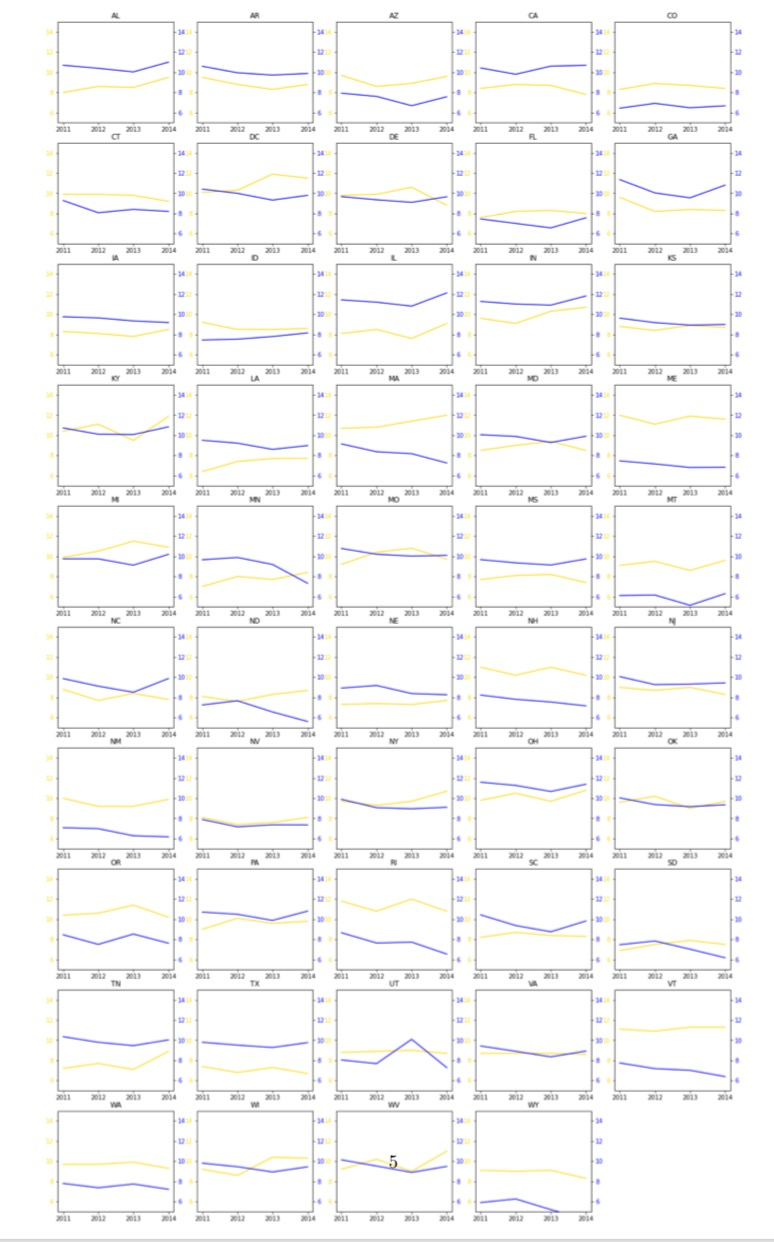
\includegraphics[width=1.0\textwidth]{Asthma-State and Year.png}
\end{figure}

\begin{figure}[h]
\centering
\caption{\label{fig:figure21}Asthma Prevalence and Gender}
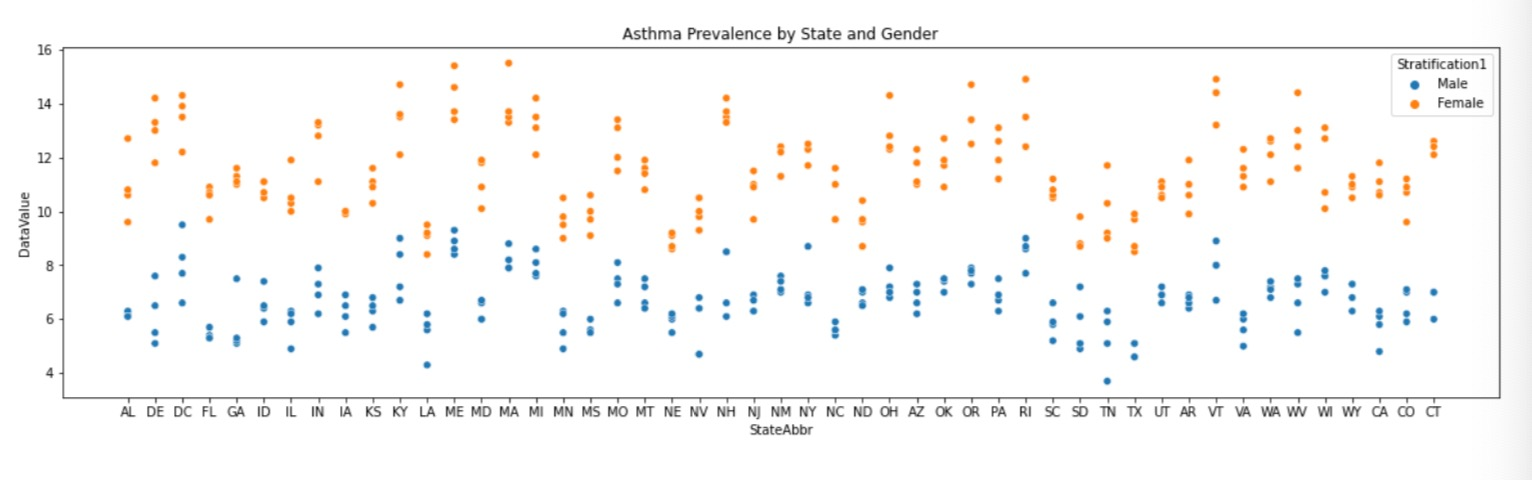
\includegraphics[width=1.0\textwidth]{Asthma Prevalence and Gender.png}
\end{figure}

\begin{figure}[h]
\centering
\caption{\label{fig:figure22}Asthma Mortality and Gender}
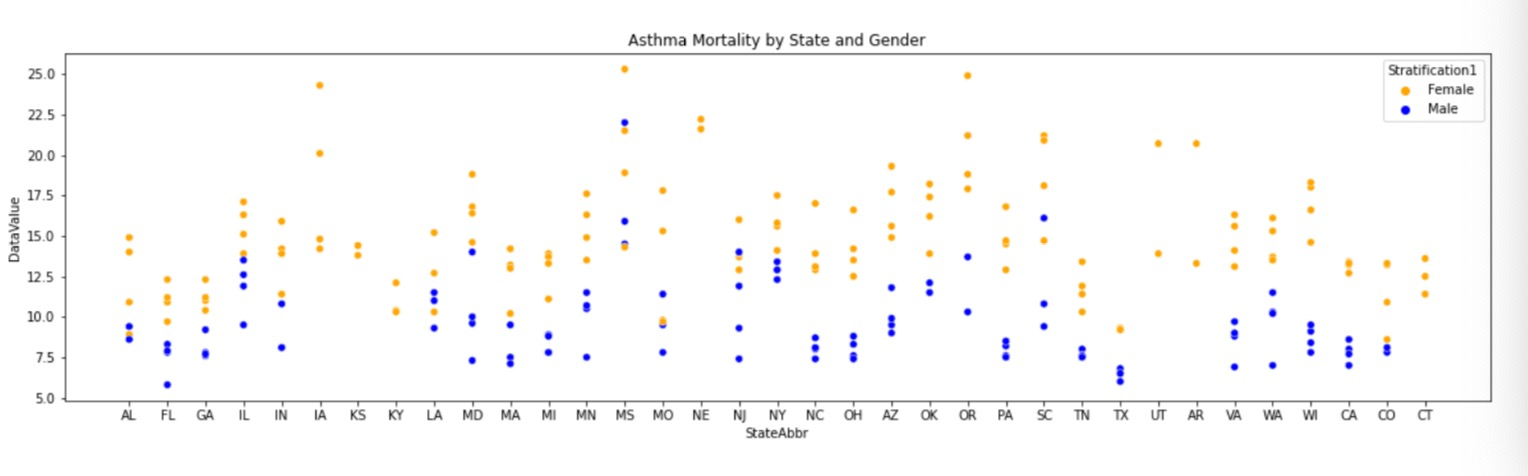
\includegraphics[width=1.0\textwidth]{Asthma Mortality and Gender.png}
\end{figure}

\begin{figure}[h]
\centering
\caption{\label{fig:figure23}Asthma Prevalence and Race}
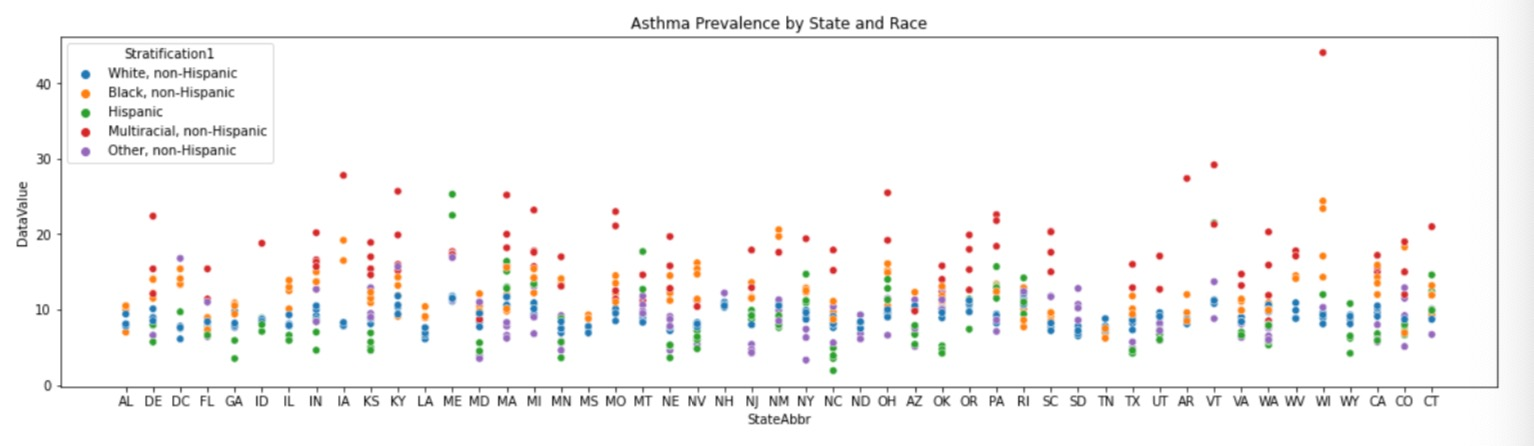
\includegraphics[width=1.0\textwidth]{Asthma Prevalence and Race.png}
\end{figure}

\begin{figure}[h]
\centering
\caption{\label{fig:figure24}Asthma Mortality and Race}
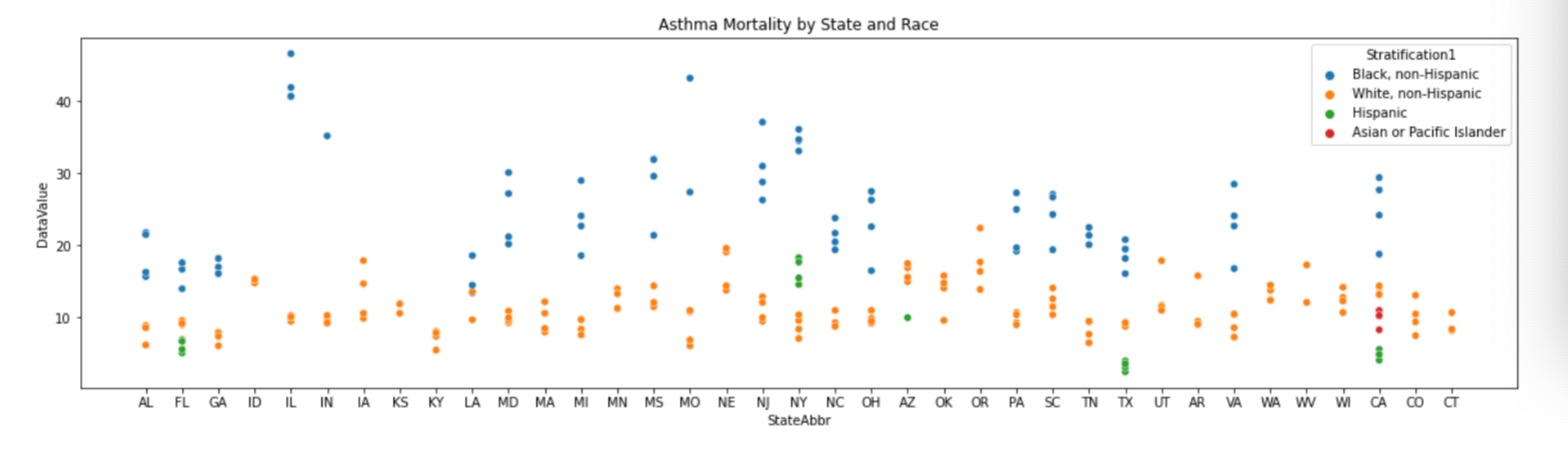
\includegraphics[width=1.0\textwidth]{Asthma Mortality and Race.png}
\end{figure}

\begin{figure}[h]
\centering
\caption{\label{fig:figure25}Latitude and Asthma Prevalence}
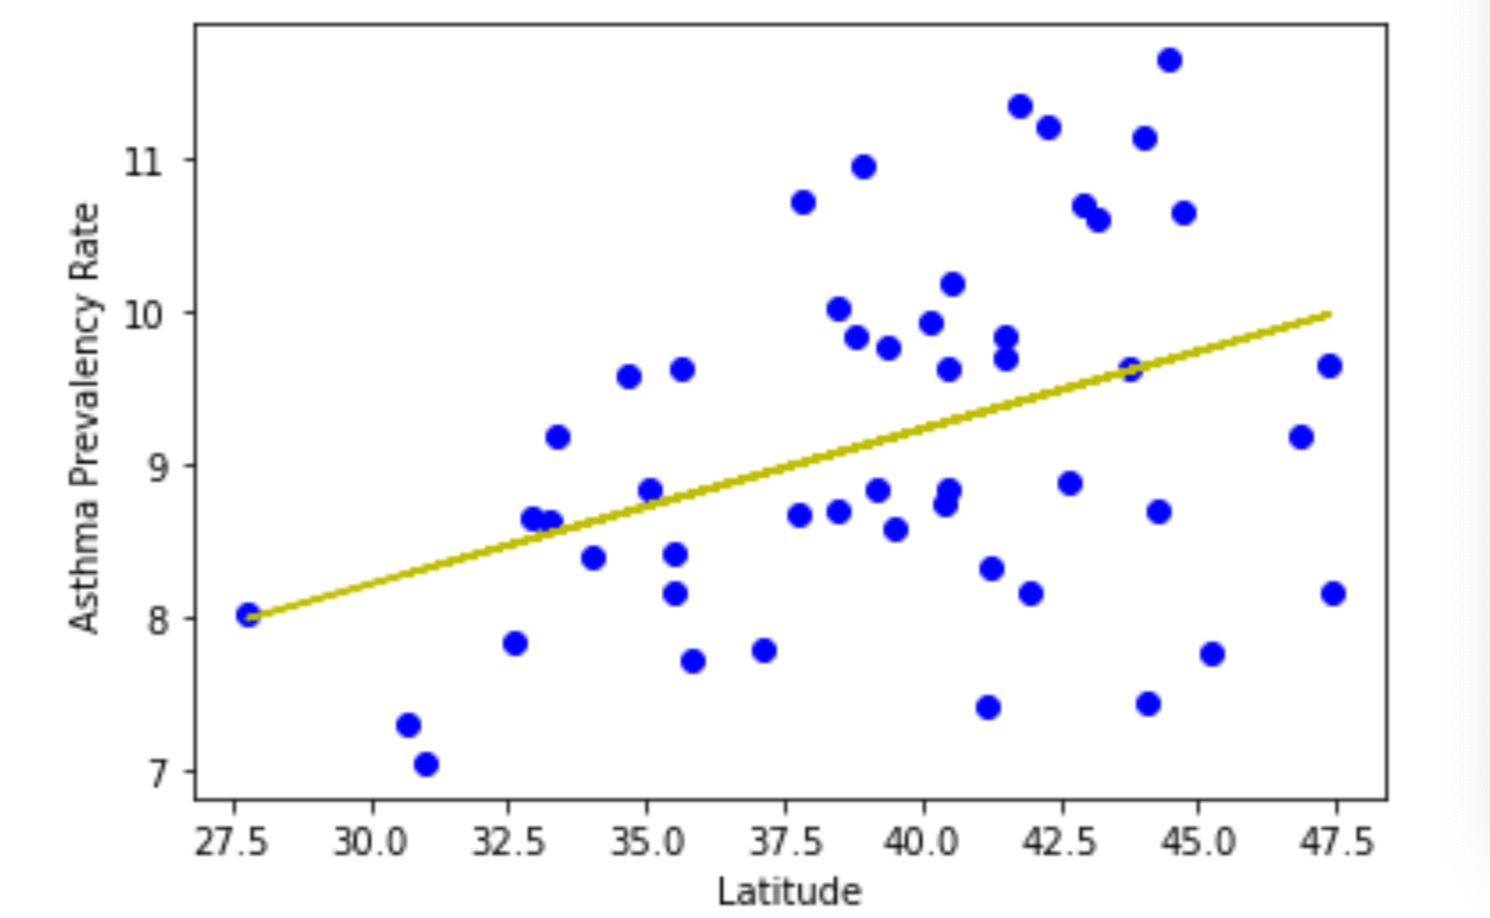
\includegraphics[width=1.0\textwidth]{Latitude and Asthma Prevalence.png}
\end{figure}

\begin{figure}[h]
\centering
\caption{\label{fig:figure26}Latitude and PM2.5}
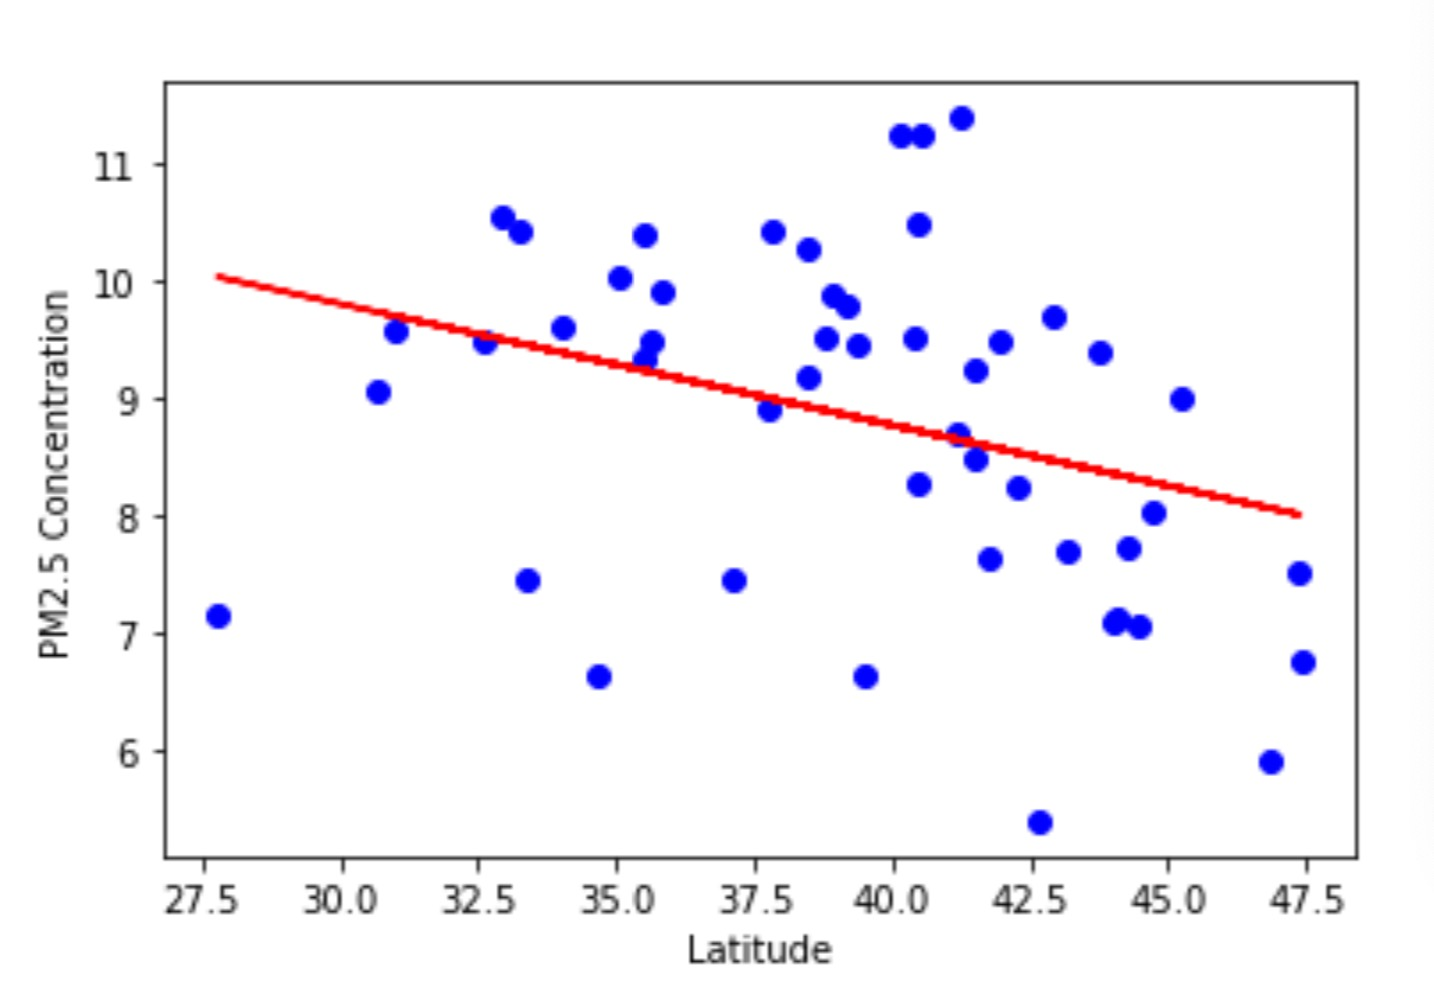
\includegraphics[width=1.0\textwidth]{Latitude and PM2.5.png}
\end{figure}

\begin{figure}[h]
\centering
\caption{\label{fig:figure1} Overall Cardiovascular Mortality by State and Year}
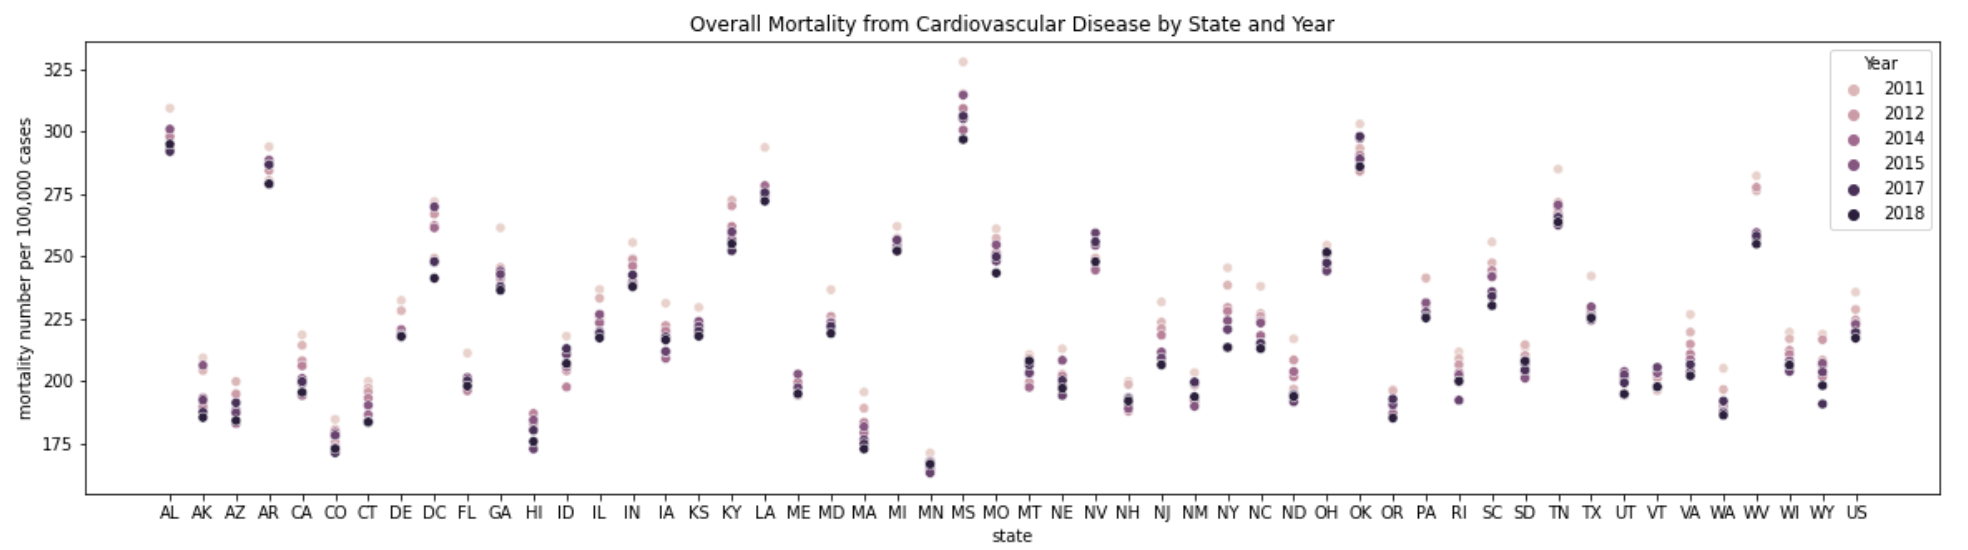
\includegraphics[width=1.0\textwidth]{mortality_cardi_graph1.png}
\end{figure}

\begin{figure}[h]
\centering
\caption{\label{fig:figure2}Cardiovascular Mortality by States Conditioned on License Policy and Year}
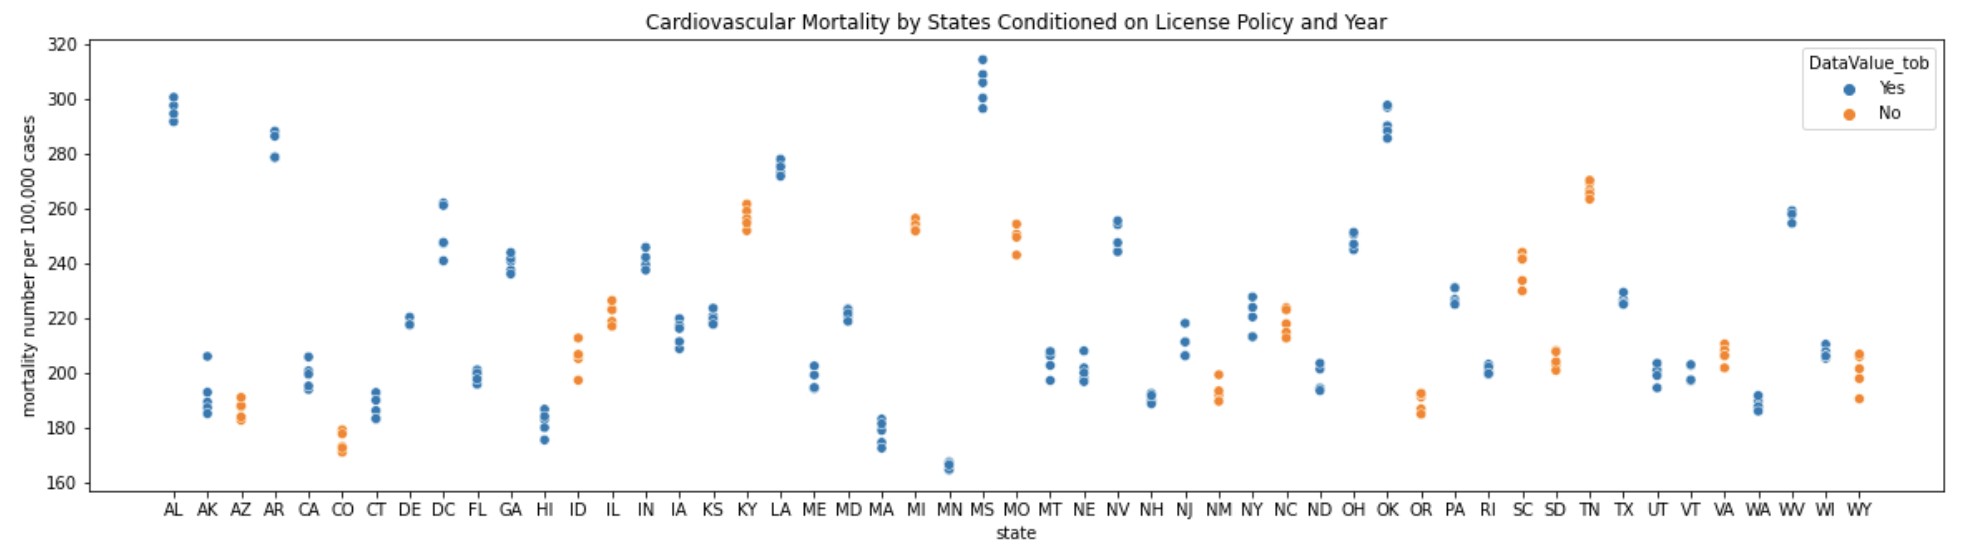
\includegraphics[width=1.0\textwidth]{mortality_toba_graph1.png}
\end{figure}

\begin{figure}[h]
\centering
\caption{\label{fig:figure3}Tobacco Usage by States and Year}
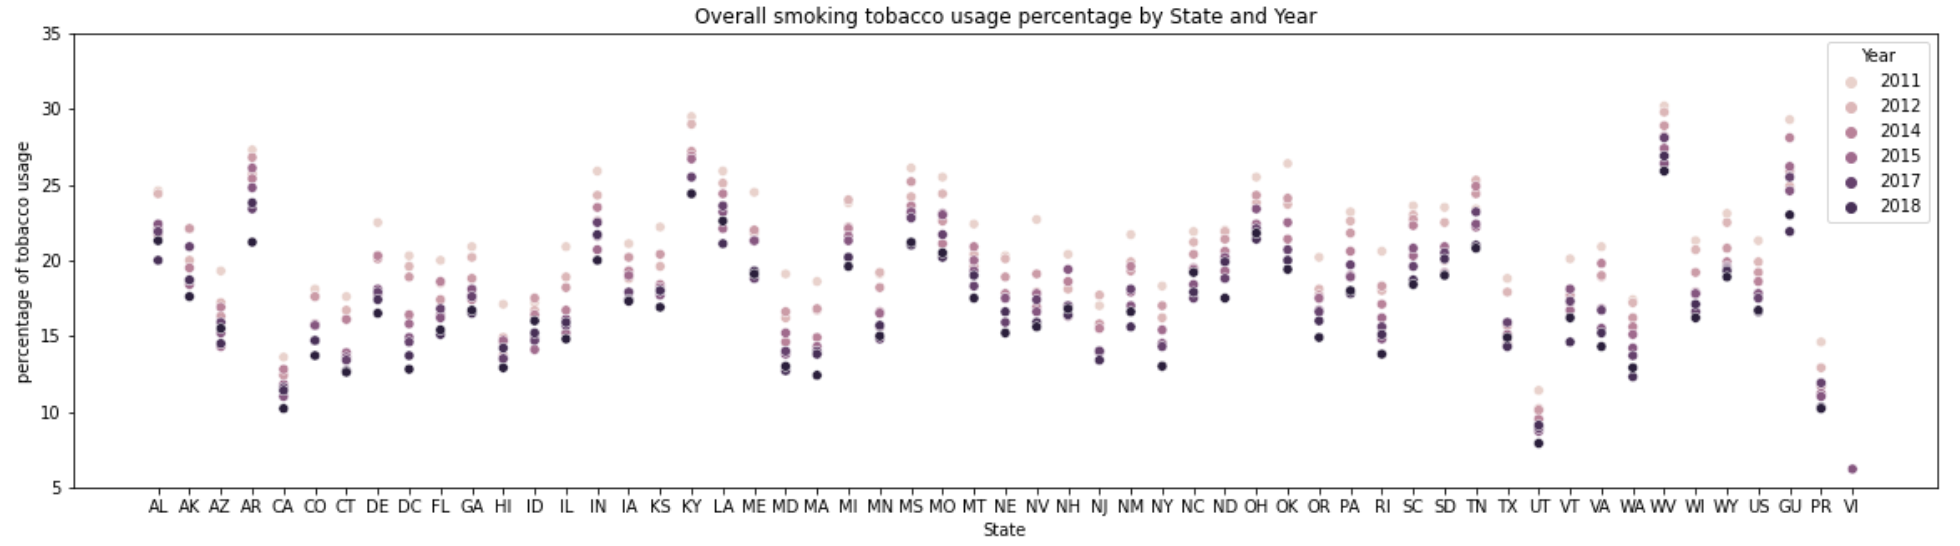
\includegraphics[width=1.0\textwidth]{toba_graph2.png}
\end{figure}


\begin{figure}
\centering
\caption{\label{fig:figureset}Mortality and Smoking Percentage by State and Year}
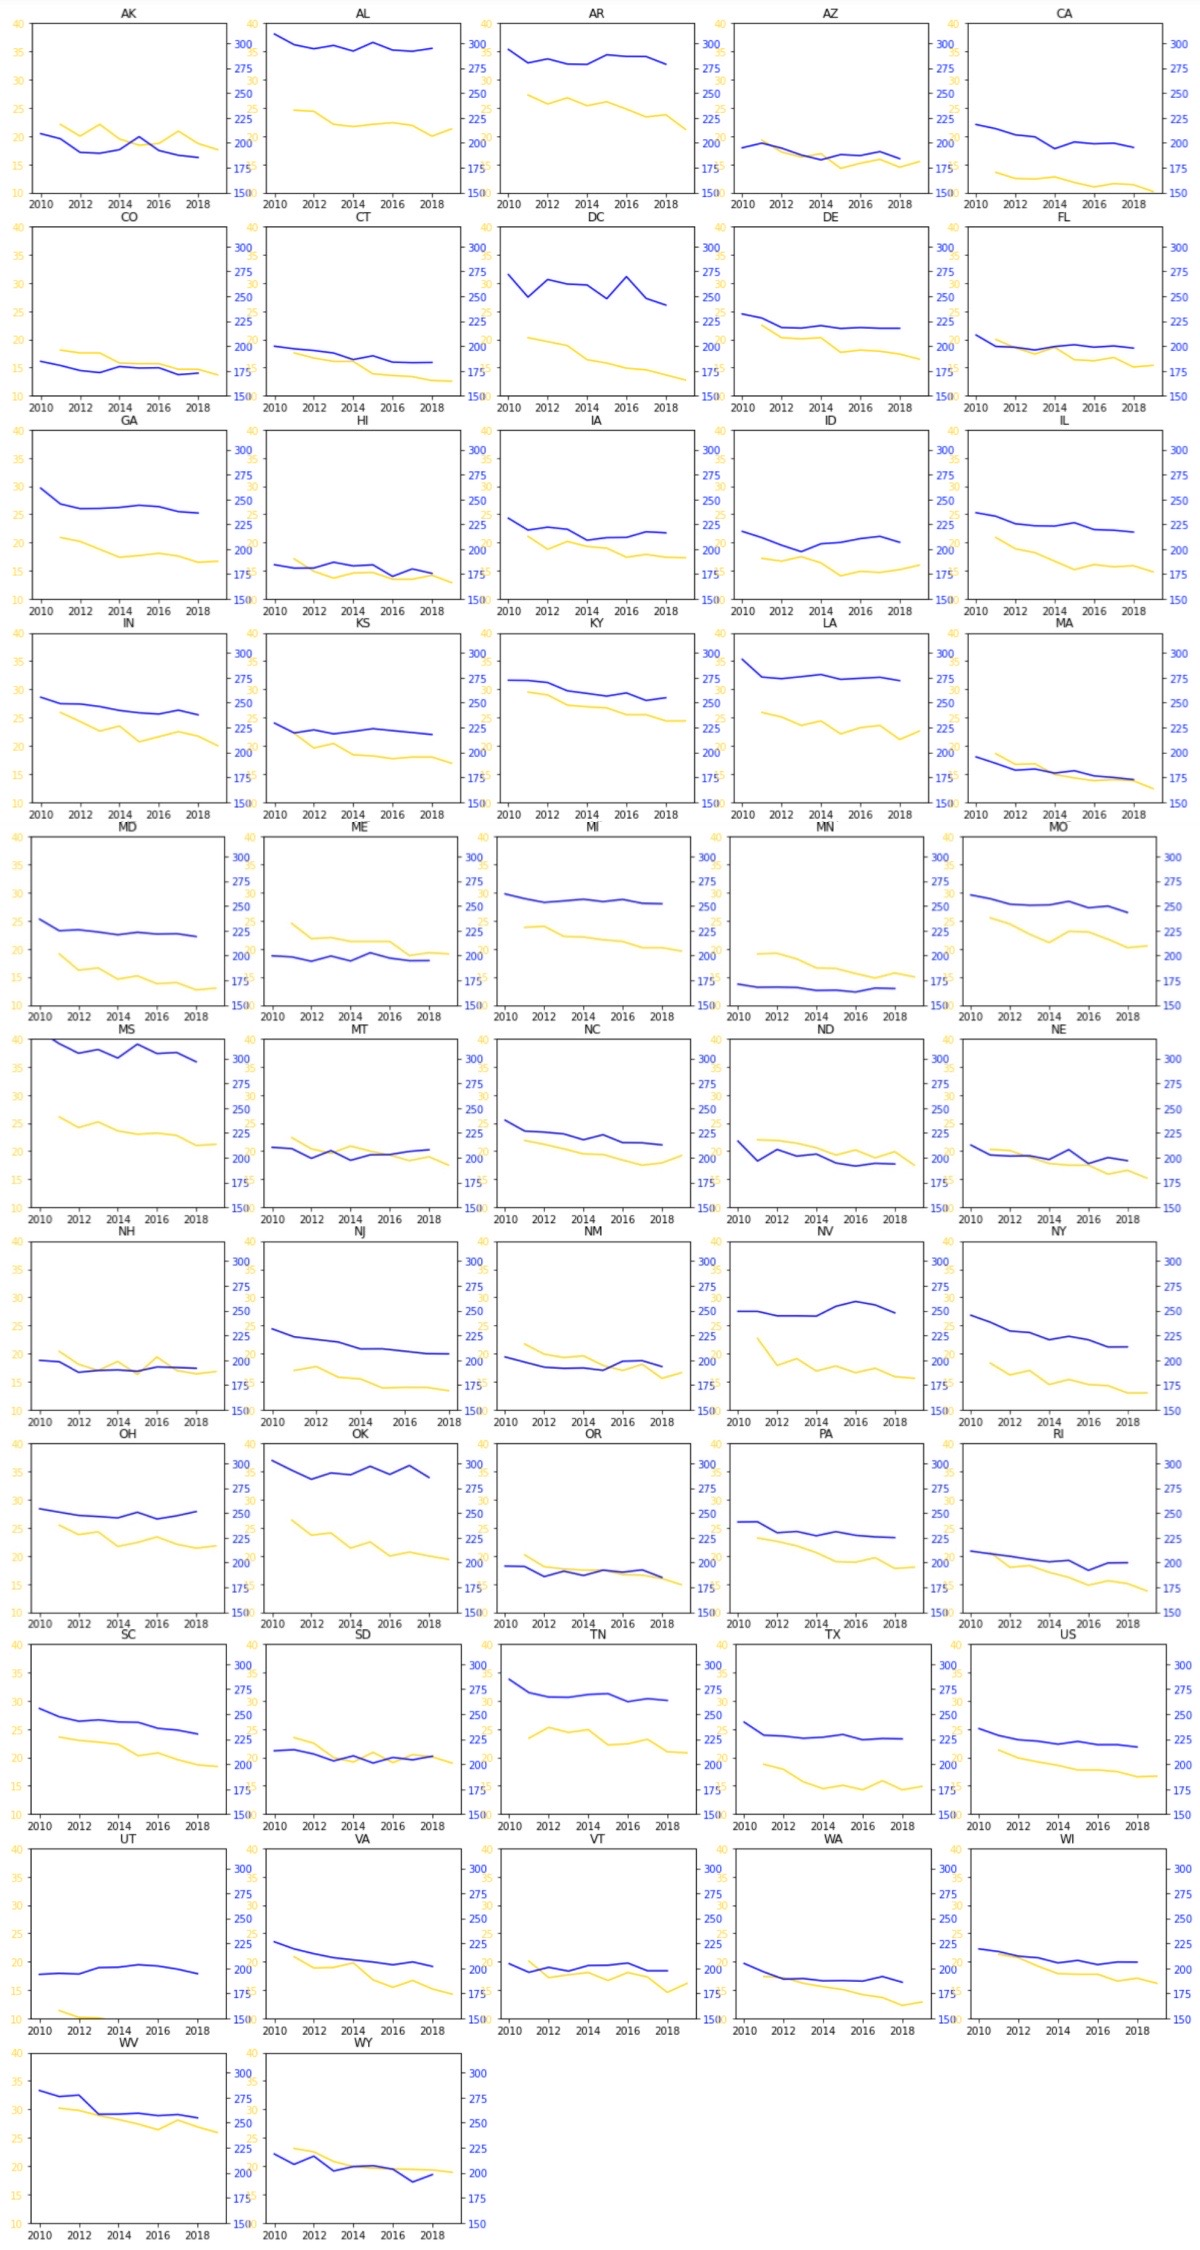
\includegraphics[width=0.8\textwidth]{set_graph1.jpg}
\end{figure}

\begin{figure}
\raggedright
\begin{minipage}{0.4\textwidth}
  \centering
  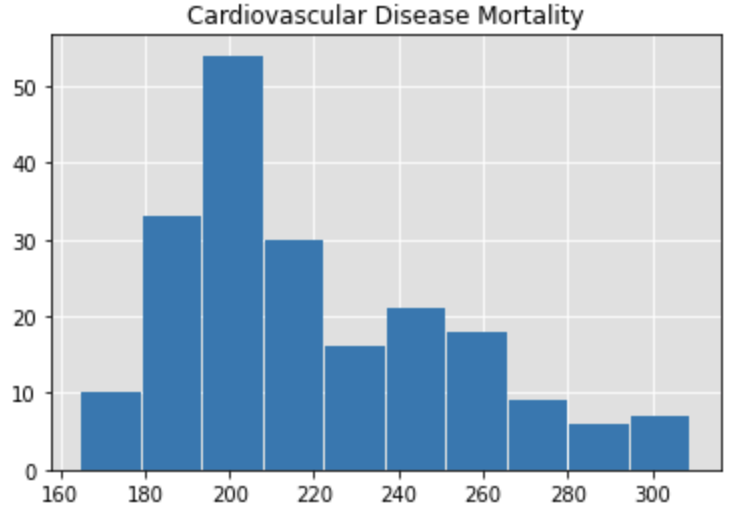
\includegraphics[width=1\linewidth]{hist1.png}
  \caption{Cardiovascular Mortality Histogram}
  \label{fig:figure5}
  
\end{minipage}%
\begin{minipage}{0.4\textwidth}
  \centering
  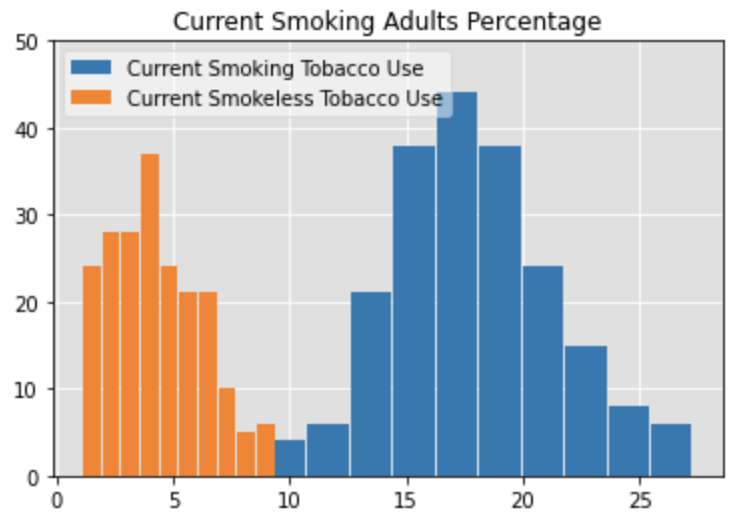
\includegraphics[width=1\linewidth]{hist2.png}
  \caption{Current Smoking Adults Percentage Histogram}
  \label{fig:figure6}
\end{minipage}
\end{figure}

\begin{figure}
\raggedright
\begin{minipage}{0.4\textwidth}
  \centering
  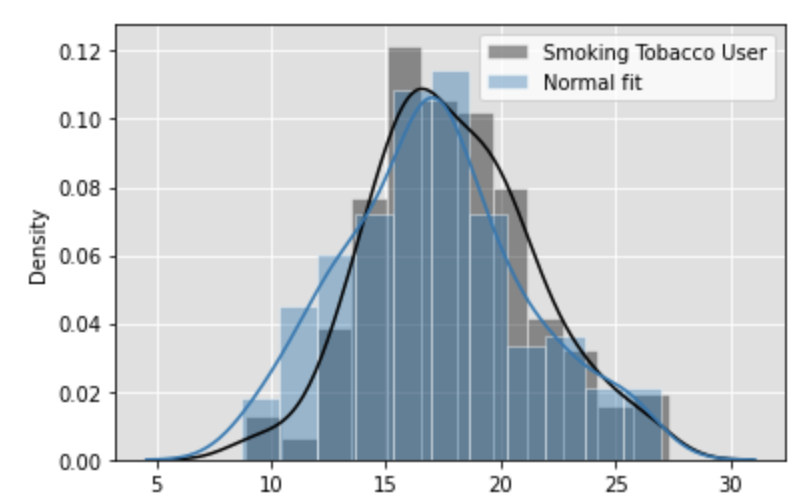
\includegraphics[width=1\linewidth]{tob1_2.png}
  \caption{Histogram of Current Adult Smoking Use}
  \label{fig:figure7}
  
\end{minipage}%
\begin{minipage}{0.4\textwidth}
  \centering
  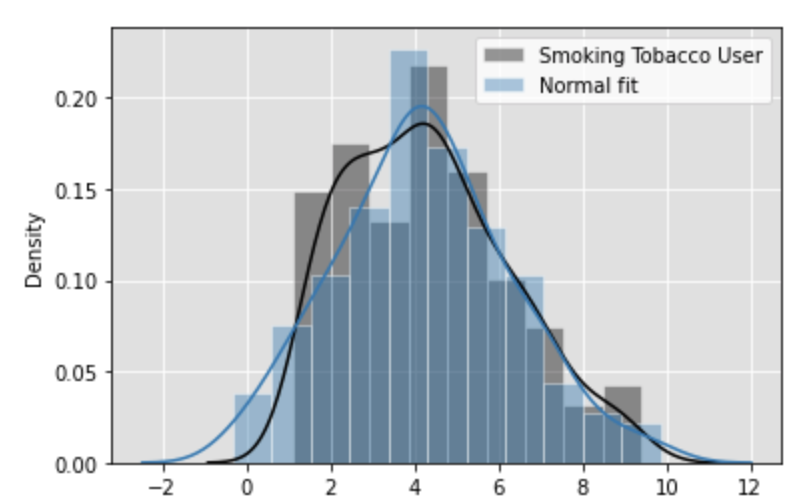
\includegraphics[width=1\linewidth]{tob2_2.png}
  \caption{Histogram of Current Adult Smokeless Tobacco Use}
  \label{fig:figure8}
\end{minipage}
\end{figure}

\begin{figure}
\raggedright
\begin{minipage}{0.4\textwidth}
  \centering
  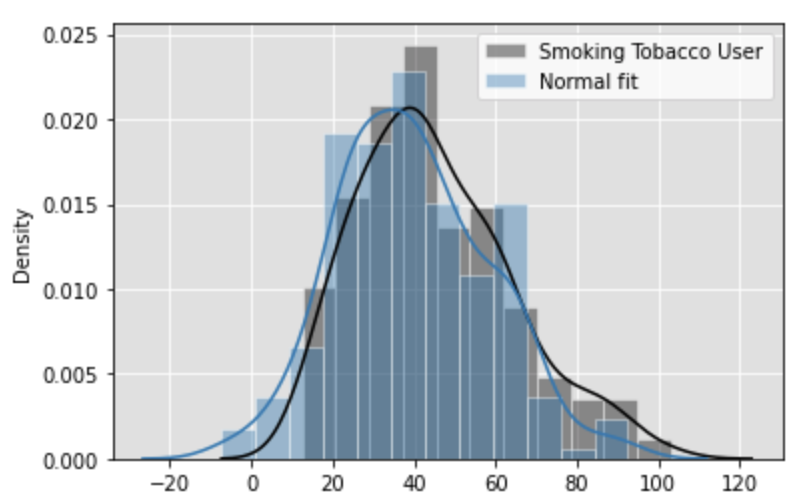
\includegraphics[width=1\linewidth]{tob10_2.png}
  \caption{Histogram of Sales of Tobacco Packs}
  \label{fig:figure9}
\end{minipage}%
\end{figure}

\begin{figure}
\centering
\begin{minipage}{0.5\textwidth}
  \centering
  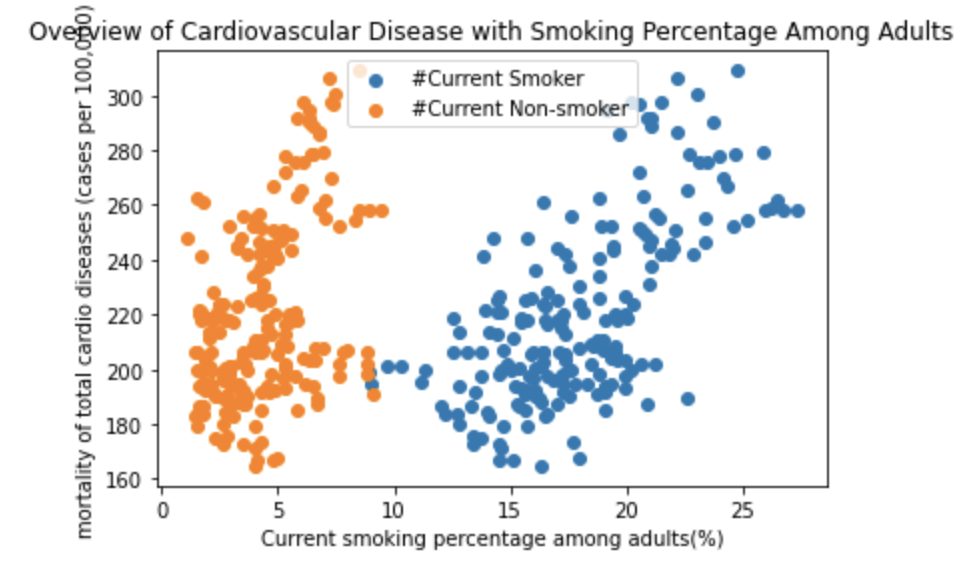
\includegraphics[width=1\linewidth]{scatter1.png}
  \caption{Cardiovascular Mortality v. Smoking Adult Percentage Conditioned on Smoker and Nonsmoker(Smokeless Tobacco)}
  \label{fig:figure10}
  
\end{minipage}%
\begin{minipage}{0.5\textwidth}
  \centering
  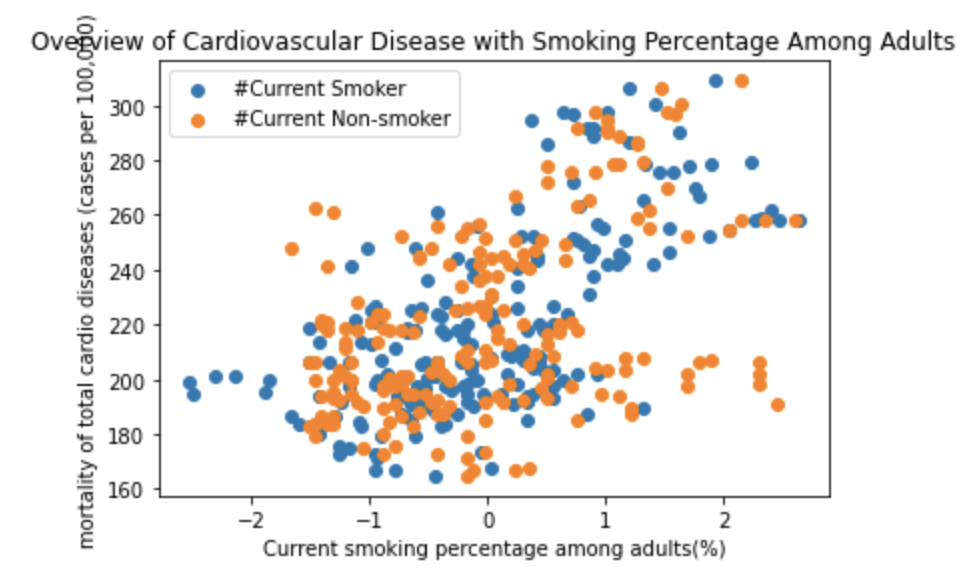
\includegraphics[width=1\linewidth]{scatter2.png}
  \caption{Standardized: Cardiovascular Mortality v. Smoking Adult Percentage Conditioned on Smoker and Nonsmoker(Smokeless Tobacco)}
  \label{fig:figure11}
\end{minipage}
\end{figure}

\begin{figure}
\centering
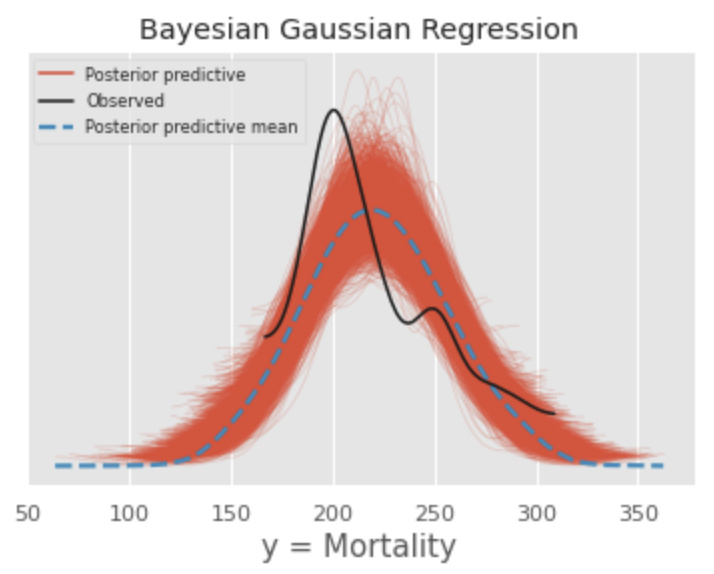
\includegraphics[width=0.5\textwidth]{gaussian_ppc.png}
\caption{Posterior Predictive Check for Bayesian Gaussian GLM}
\label{fig:figure12}
\end{figure}

\begin{figure}
\centering
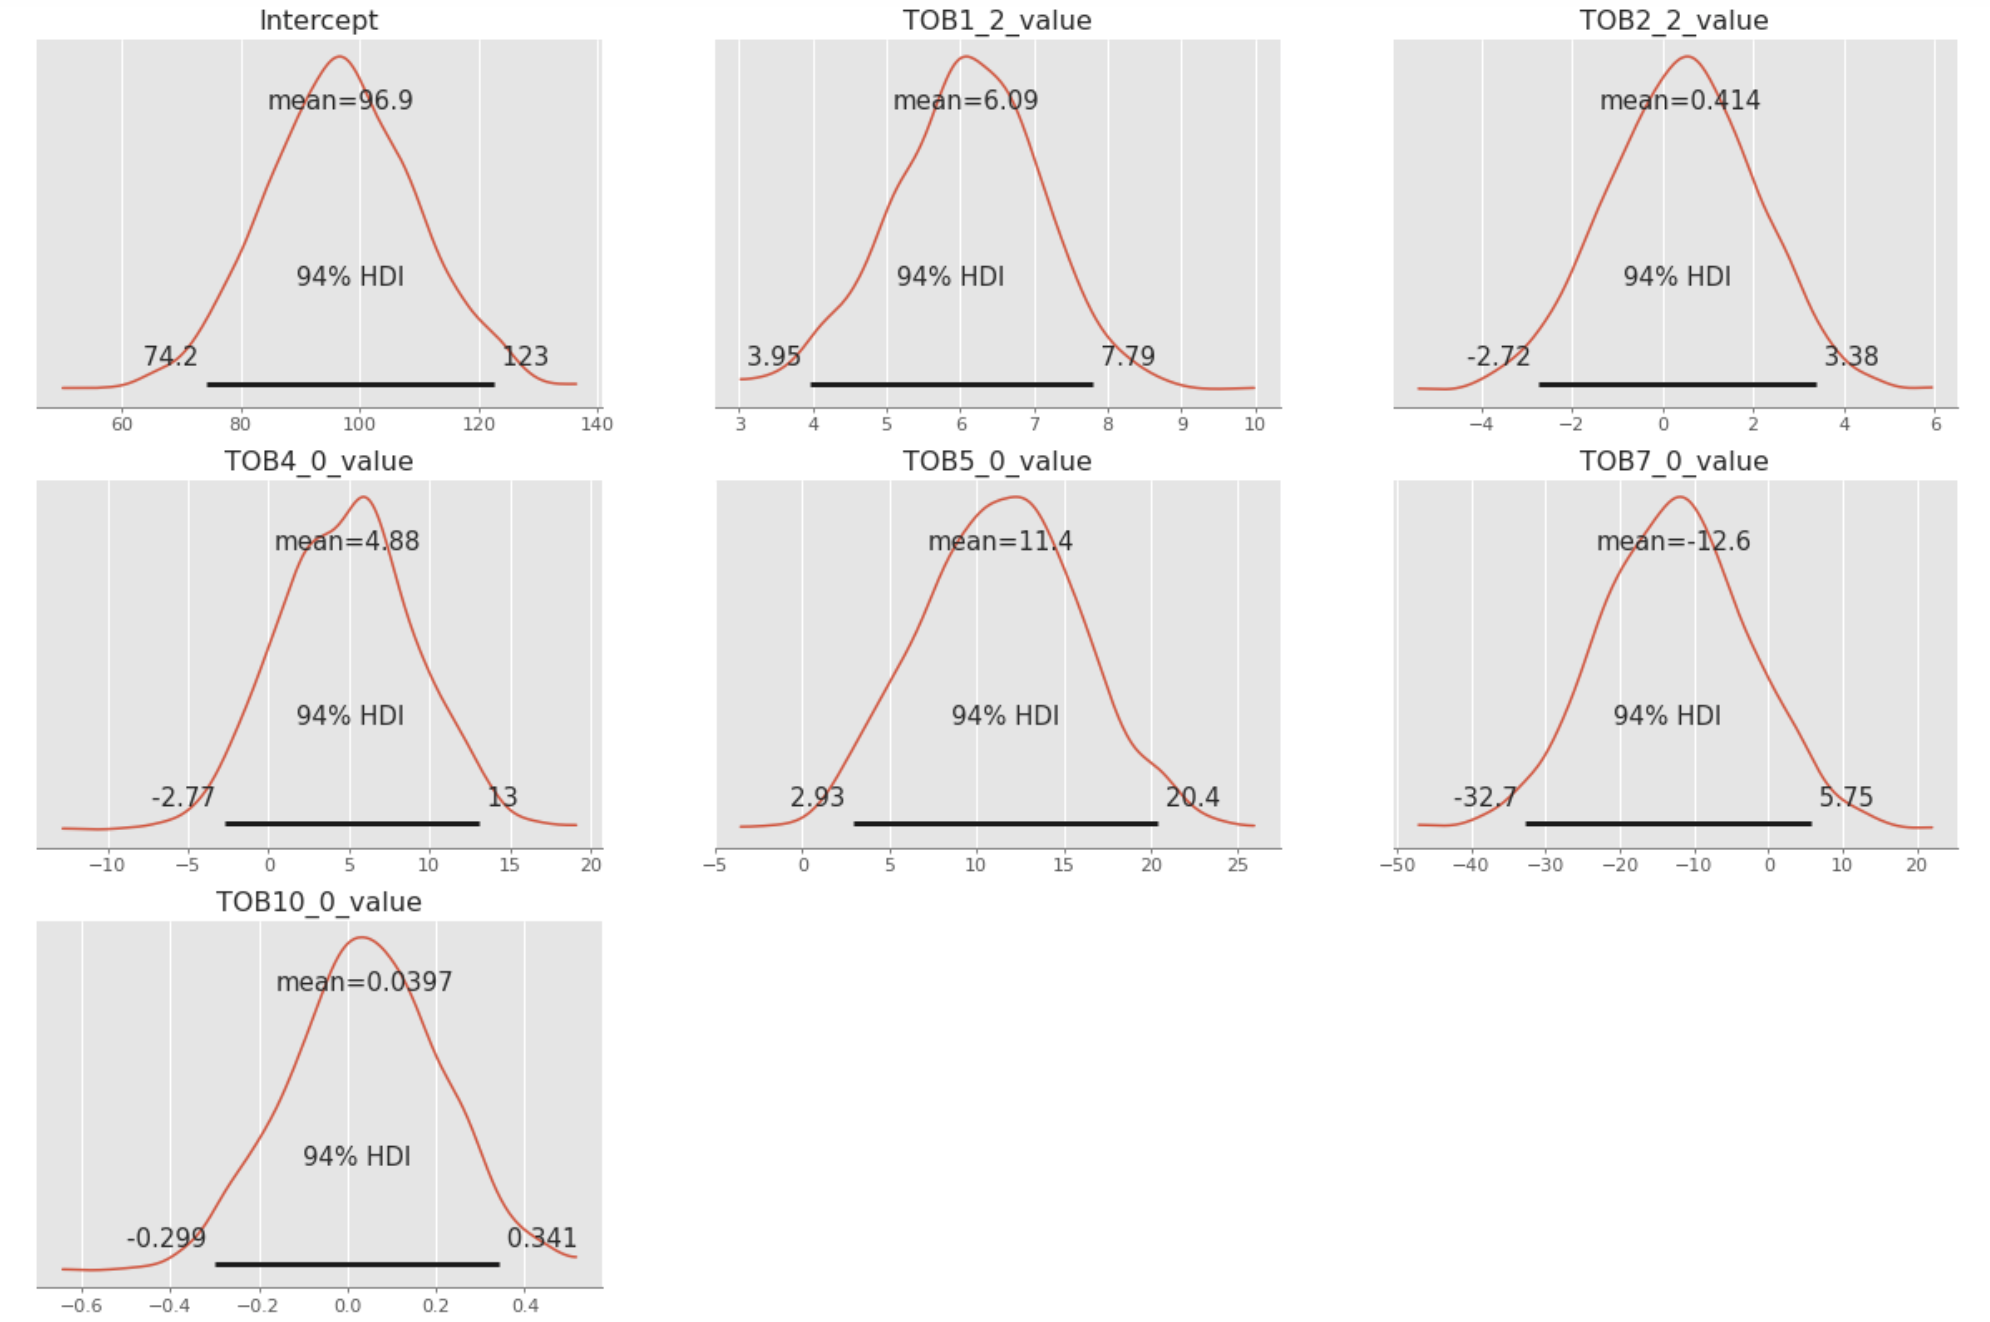
\includegraphics[width=1.0\textwidth]{gaussian_pos.png}
\caption{Coefficient Credible Intervals for Bayesian Gaussian GLM}
\label{fig:figure13}
\end{figure}

\begin{figure}
\centering
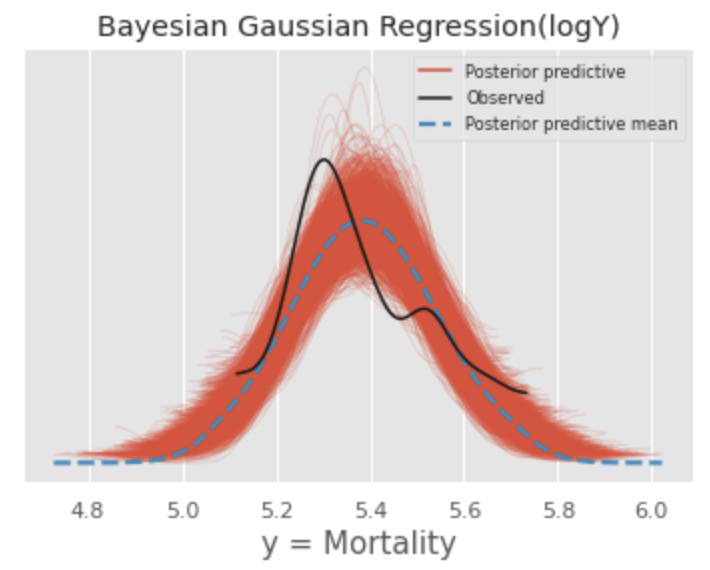
\includegraphics[width=0.5\textwidth]{gaussian_logy_ppc.png}
\caption{Posterior Predictive Check for Bayesian Gaussian GLM with Log(y)}
\label{fig:figure14}
\end{figure}

\begin{figure}
\centering
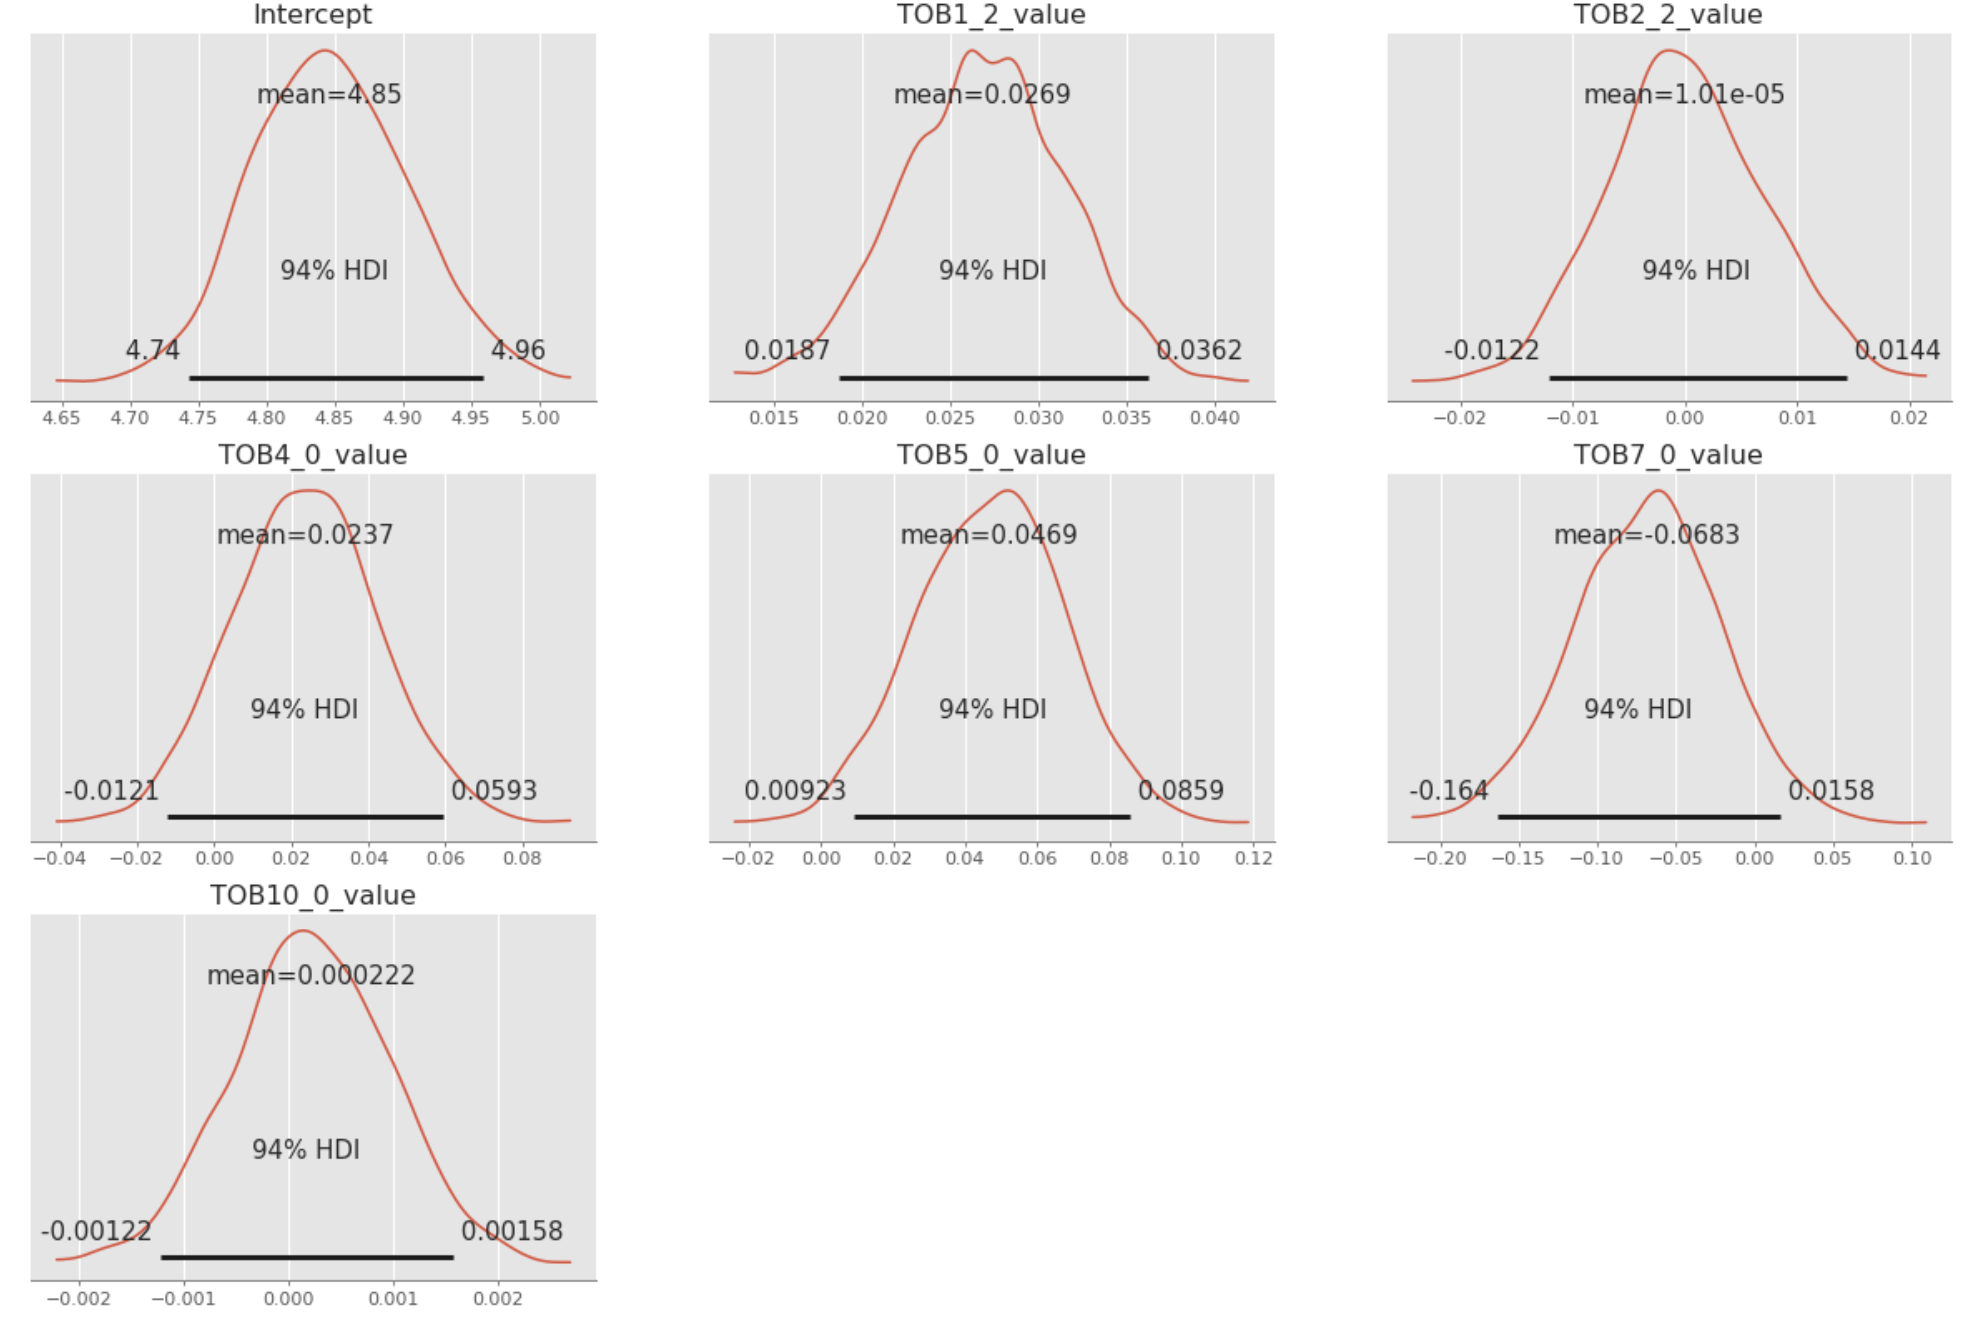
\includegraphics[width=1.0\textwidth]{gaussian_logy_pos.png}
\caption{Coefficient Credible Intervals for Bayesian Gaussian GLM with Log(y)}
\label{fig:figure15}
\end{figure}

\begin{figure}
\centering
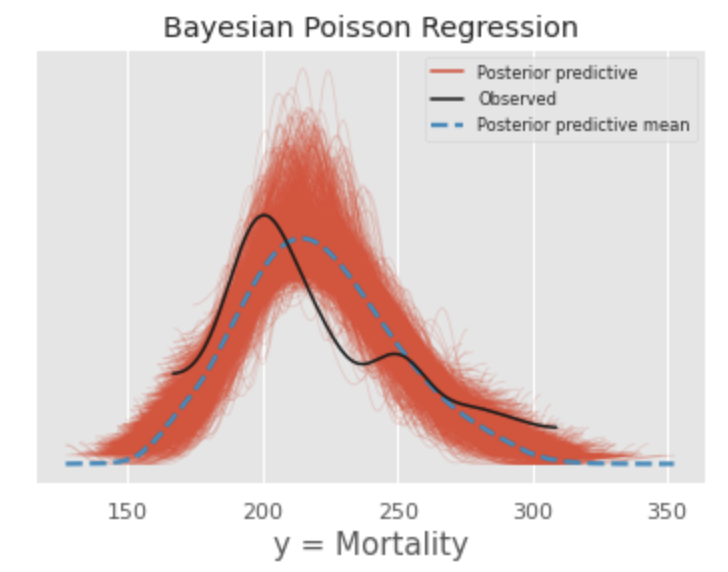
\includegraphics[width=0.5\textwidth]{poisson_ppc.png}
\caption{Posterior Predictive Check for Bayesian Poisson GLM}
\label{fig:figure16}
\end{figure}

\begin{figure}
\centering
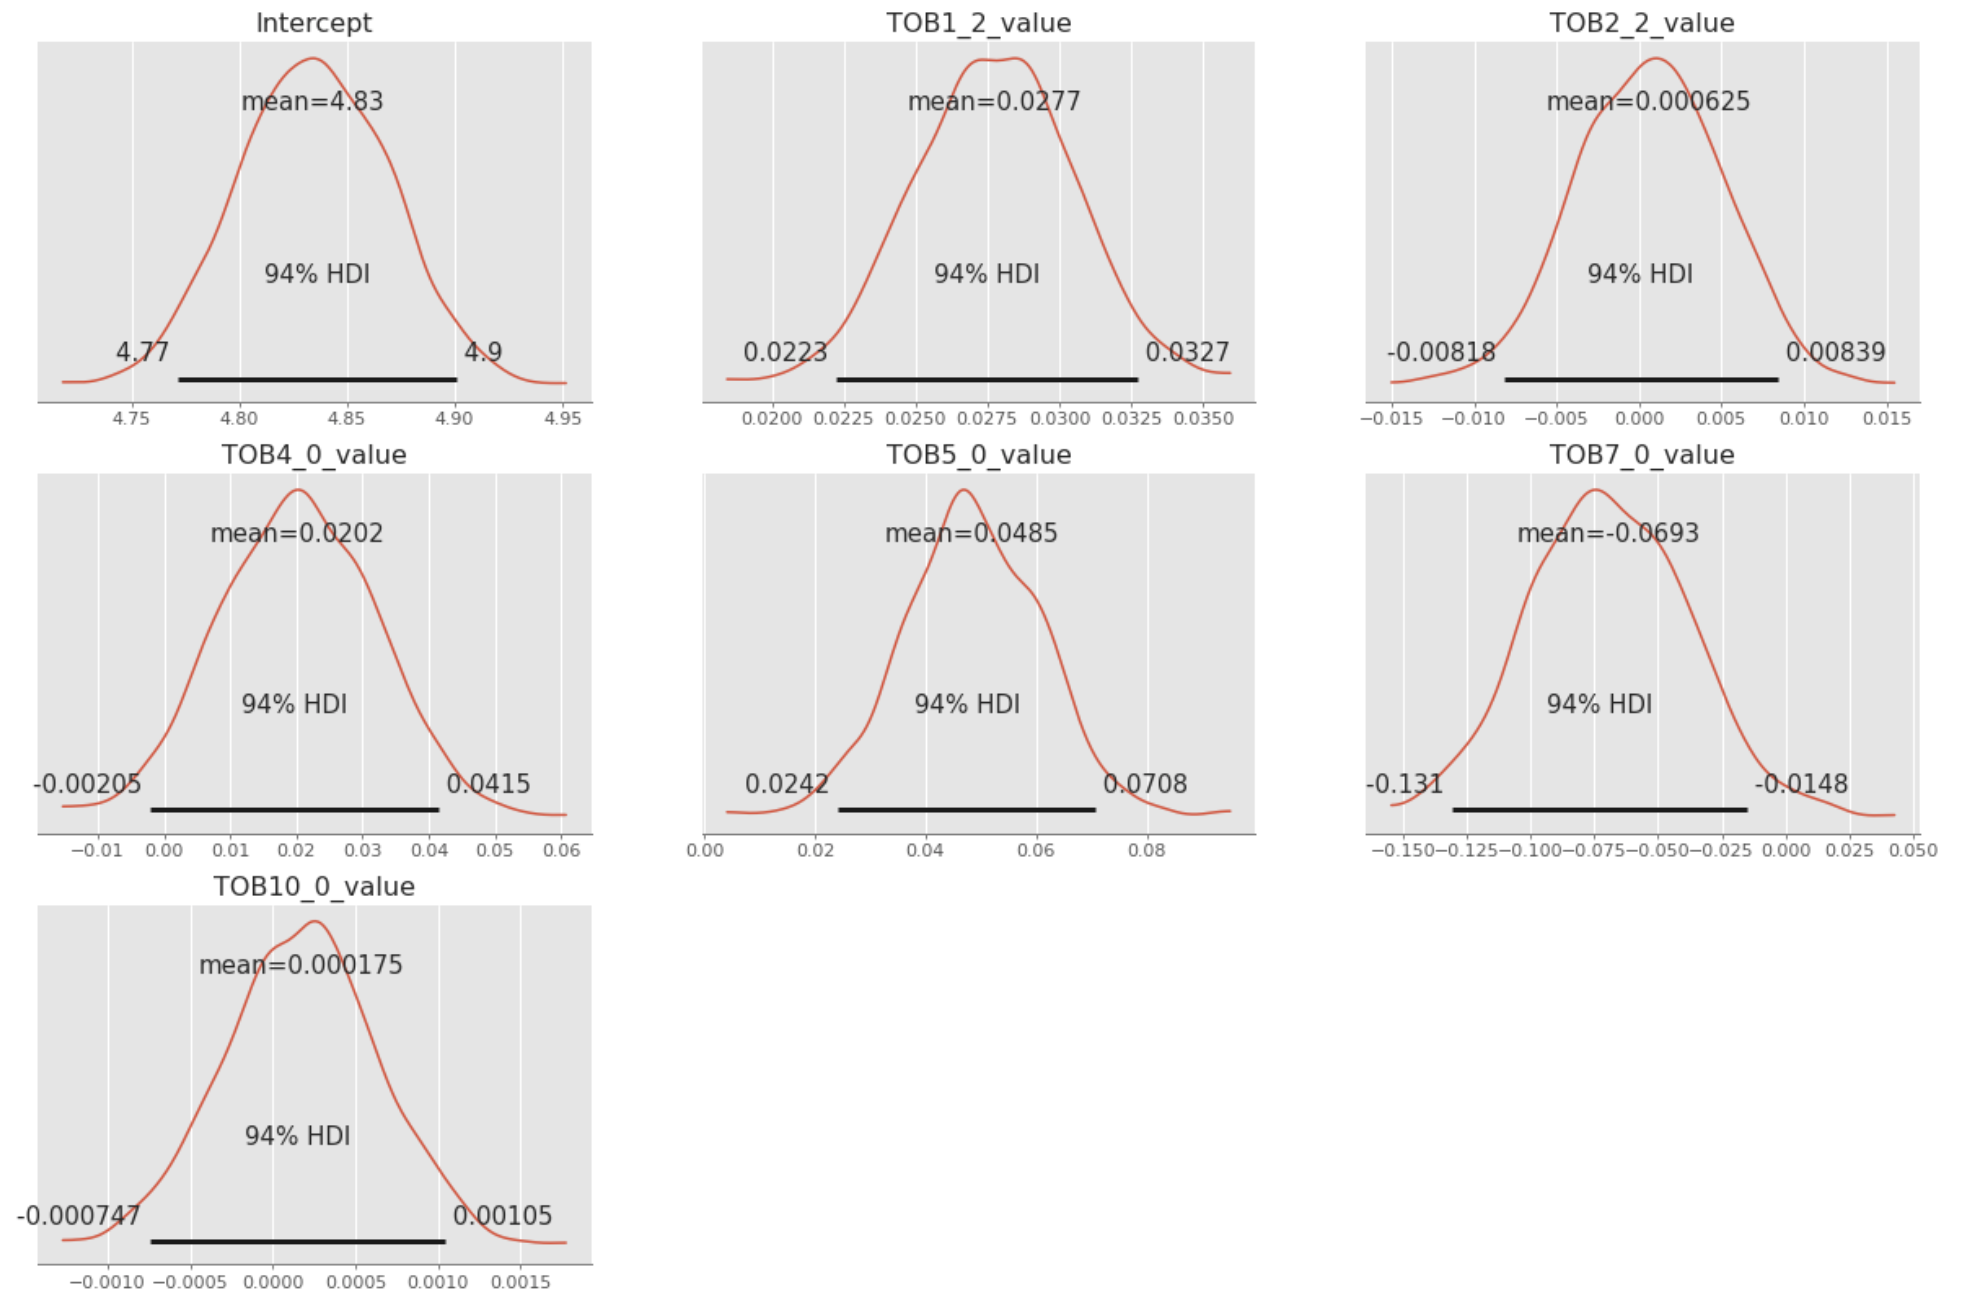
\includegraphics[width=1.0\textwidth]{poisson_pos.png}
\caption{Coefficient Credible Intervals for Bayesian Poisson GLM}
\label{fig:figure17}
\end{figure}

\begin{figure}
\centering
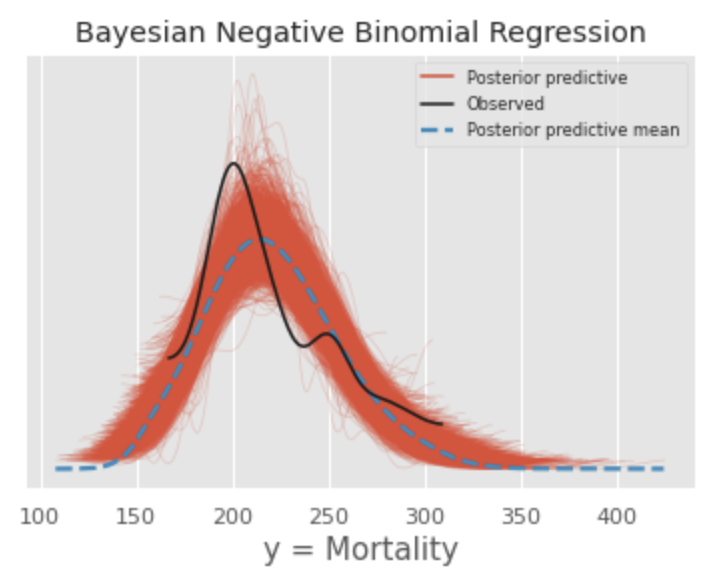
\includegraphics[width=0.5\textwidth]{nb_ppc.png}
\caption{Posterior Predictive Check for Bayesian Negative Binomial GLM}
\label{fig:figure18}
\end{figure}

\begin{figure}
\centering
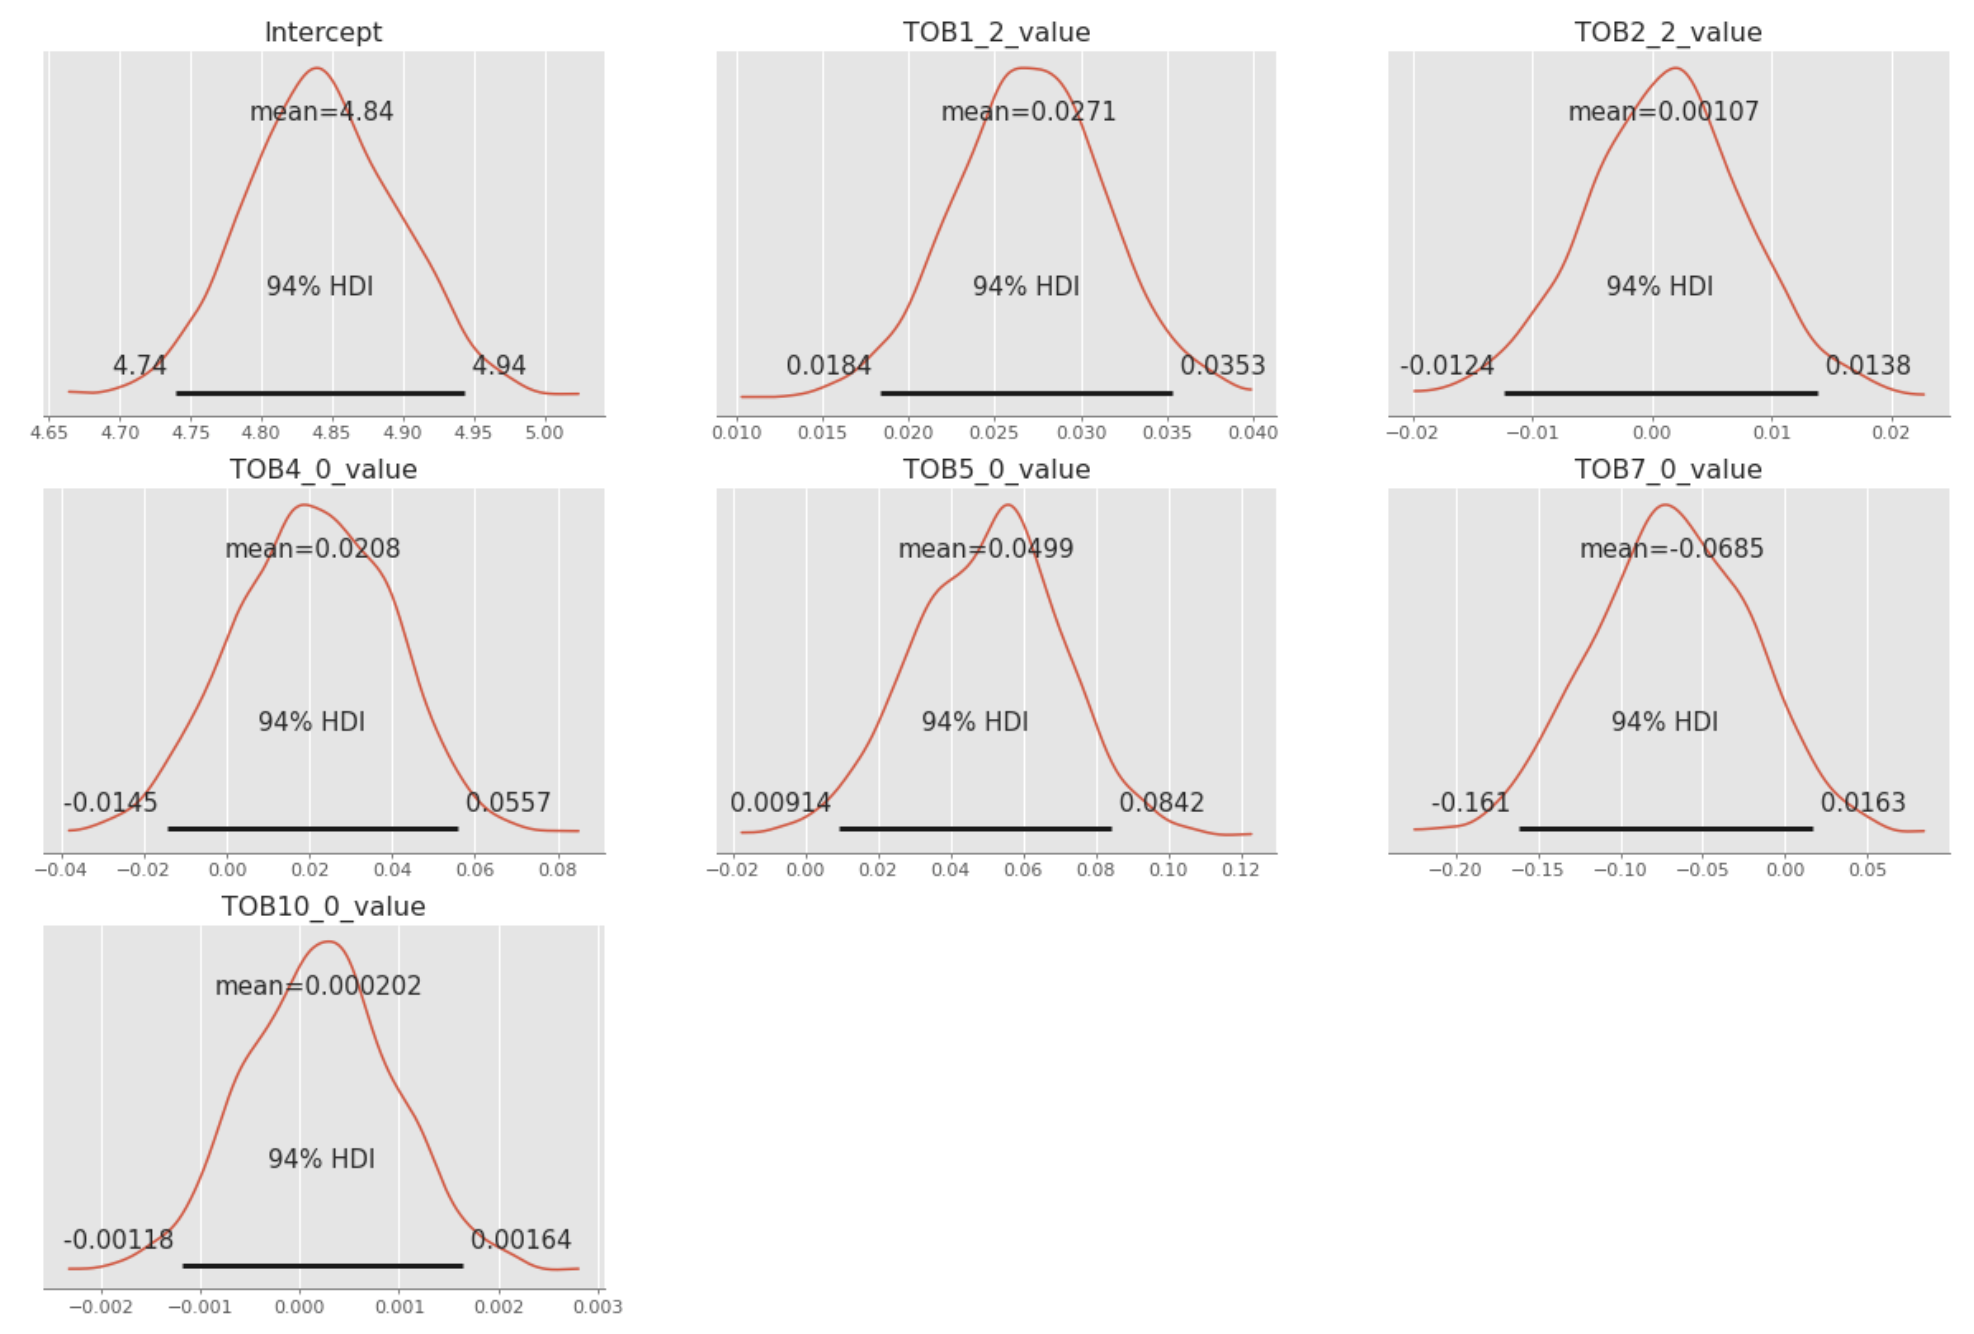
\includegraphics[width=1.0\textwidth]{nb_pos.png}
\caption{Coefficient Credible Intervals for Bayesian Negative Binomial GLM}
\label{fig:figure19}
\end{figure}


\end{document}